\chapter{Reduction Formula of Kampé de Fériet function}


\label{ch_5}
\hspace{\parindent}

From chapter \ref{ch_3}, we see how the summation involving digamma function naturally arises in the calculation of the finite-part integral, specifically in the case of pole singularity. While in chapter \ref{ch_4}, we obtain the relation of this summation to the reduction formula of Kampé de Fériet function. In this chapter, we will exploit the result of the exact evaluation of the Stieltjes transform and use the established relation from the previous chapter to tabulate reduction formulas of the Kampé de Fériet function. 

All of the theorems and corollaries presented in this chapter were numerically verified. Numerical verification means that both side of the equation will be evaluated numerically for a random set of parameters and compare their numerical values. The equality holds if both right hand sides of the equation agree to the same numerical value. The code in Mathematica notebook used in the numerical verification can be found in the Appendix \ref{mathematica}. The code with $10$ digits of precision were executed on the following specifications: Intel i5-9300H processor CPU @ 2.40 GHz and 16GB RAM. The code were all written in Wolfram Mathematica v12.1.

\section{Reduction formula from Generalized Stieltjes transform of $f(x) = e^{-bx}$}

According to \cite{erdelyi1954tables}, the generalized Stietljes transform of $f(x) = e^{-bx}$ for integral order is known to be 
\begin{equation} \label{5.1}
    \int_0^{\infty} \frac{e^{-bx}}{(\omega + x)^{n}} \, \mathrm{d}x = b^{n-1}e^{b\omega} \, \Gamma(1-n,\, b\omega),
\end{equation}
for $\mathrm{Re}(b)>0$ and $|\mathrm{arg}(\omega)|>\pi$. The $\Gamma(s,x)$ factor refers to the incomplete gamma function, which is expressed as
\begin{equation}
    \Gamma(s,x) = \int_{x}^{\infty} t^{s-1} \, e^{-t} \, \mathrm{d}t.
\end{equation} 
The integral will be evaluated using the method of finite-part integration. Obviously, when we expand the kernel, we will have a pole singularity. Therefore, we will use Theorem \ref{T3.3} to evaluate the integral. Invoking the theorem, we will have the expression
\begin{equation} \label{5.2}
    \int_0^{\infty} \frac{e^{-bx}}{(\omega + x)^{n}} \mathrm{d}t = \sum_{k=0}^{\infty} \binom{-n}{k} \omega^{k} \bbint{0}{\infty} \frac{e^{-bx}}{x^{k+n}} \, \mathrm{d}x + \Delta_{\mathrm{sc}}^{(n)}(\omega).
\end{equation}
where 
\begin{equation}
\begin{split} \label{sc4.1}
    \Delta_{\mathrm{sc}}^{(n)}(\omega) & =  -\frac{\ln{\omega}}{\Gamma(n)} \left. \frac{\mathrm{d}^{n-1}}{\mathrm{d}z^{n-1}} \,  e^{-bz} \right|_{z=-\omega} + \sum_{k=0}^{n-2} \frac{\omega^{k-n+1}}{k!(n-1-k)} \left. \frac{\mathrm{d}^{k}}{\mathrm{d}z^{k}} \,  e^{-bz} \right|_{z=-\omega} 
    \\& = -\frac{\ln{\omega}}{\Gamma(n)} (-b)^{n-1} e^{b\omega} + \sum_{k=0}^{n-2} \frac{\omega^{k-n+1}}{k!(n-1-k)} (-b)^{k} e^{b\omega}
\end{split}
\end{equation}
Using the tabulated list of evaluated finite-part integral in \cite{ticathetit}, the finite-part integral from the above equation is calculated to be
\begin{equation}
    \bbint{0}{\infty} \frac{e^{-bx}}{x^{k+n}} \, \mathrm{d}x = \frac{(-1)^{k+n} b^{k+n-1}}{\Gamma(k+n)} (\ln{b} - \psi(k+n))
\end{equation}
We will substitute the evaluated finite-part integral and equation \eqref{sc4.1} to equation \eqref{5.2}. Then, we will rewrite the combination in terms of gamma function and express the summation of digamma function as ${}_p\tilde{\psi}_{q}$ using equation \eqref{psi}. The desired integral will assume the form
\begin{equation}
\begin{split} \label{5.4}
    \int_0^{\infty} \frac{e^{-bx}}{(\omega + x)^{n}} = & \frac{(-1)^n \, b^{n-1}}{\Gamma(n)} \Bigg[ \sum_{k=0}^{\infty} \frac{(\omega b)^{k}}{k!} \ln{b} - \pPq{0}{0}{}{}{n}{b\omega} \Bigg]
    \\& -\frac{\ln{\omega}}{\Gamma(n)} (-b)^{n-1} e^{b\omega} + \sum_{k=0}^{n-2} \frac{\omega^{k-n+1}}{k!(n-1-k)} (-b)^{k} e^{b\omega}.
\end{split}
\end{equation}
Now, we see the infinite series with logarithmic factor can be simplified into exponential function. Combining the similar terms, we will have
\begin{equation}
\begin{split} \label{5.5}
    \int_0^{\infty} \frac{e^{-bx}}{(\omega + x)^{n}} = & -\frac{(-1)^{n} \, b^{n-1}}{\Gamma(n)} \pPq{0}{0}{}{}{n}{b\omega} - \frac{(-b)^{n-1} e^{b \omega}}{\Gamma(n)} \ln{b\omega}
    \\& - b^{n-1}\sum_{k=0}^{n-2} (-1)^{k} \frac{(b\omega)^{k-n+1}}{k!(n-1-k)} e^{b\omega}.
\end{split}
\end{equation}
Next, we will use the relation of the function ${}_p\tilde{\psi}_{q}$ to the Kampé de Fériet function express in \eqref{DxKv0} to arrive to this relation
\begin{equation} \label{5.6}
    \pPq{0}{0}{}{}{n}{b\omega} = \psi(n) e^{b\omega} + \frac{b\omega}{n} F^{-:\;1;\;2}_{1:\;-;\;1}\left[\begin{array}{ccc}
     -:& 1; & 1, n  \\
     2:& -; & n+1 
    \end{array};\;  b\omega,b\omega\right].
\end{equation}
Putting back equation \eqref{5.6} to equation \eqref{5.5} and substituting \eqref{5.1} to the left hand side of \eqref{5.5}, will yield to
\begin{equation}
\begin{split}
    b^{n-1} e^{b\omega} \,& \Gamma(1-n,\, b\omega) \\& = -\frac{(-1)^n \, b^{n-1}}{\Gamma(n)} \left(  \psi(n) e^{b\omega} + \frac{b\omega}{n} F^{-:\;1;\;2}_{1:\;-;\;1}\left[\begin{array}{ccc}
     -:& 1; & 1, n  \\
     2:& -; & n+1 
    \end{array};\;  b\omega,b\omega\right] \right) \\& - \frac{(-b)^{n-1}}{\Gamma(n)} e^{b \omega} \ln{b\omega} - b^{n-1}\sum_{k=0}^{n-2} (-1)^{k} \frac{(b\omega)^{k-n+1}}{k!(n-1-k)} e^{b\omega}.
\end{split}
\end{equation}
Simplifying it further by combining similar terms and letting $z = b\omega$ will result to
\begin{equation}
\begin{split}
     e^{z} \,& \Gamma(1-n,\, z) = -\frac{(-1)^n}{\Gamma(n)} \frac{z}{n} F^{-:\;1;\;2}_{1:\;-;\;1}\left[\begin{array}{ccc}
     -:& 1; & 1, n  \\
     2:& -; & n+1 
    \end{array};\;  z,z\right] \\& - \frac{(-1)^{n-1}}{\Gamma(n)} e^{b \omega} (\ln{z} - \psi(n)) - \sum_{k=0}^{n-2} (-1)^{k} \frac{(z)^{k-n+1}}{k!(n-1-k)} e^{z}.
\end{split}
\end{equation}
By the concept of analytic continuation, the value of $z$ extends to the complex plane. Also, the reduction formula of the Kampé de Fériet function is obtained by isolating the function. 

\begin{theorem}
For complex number $z$ and positive integer $n$ the reduction formula of the Kampé de Fériet function is equal to
\begin{equation}
\begin{split}
      F^{-:\;1;\;2}_{1:\;-;\;1}\left[\begin{array}{ccc}
     -:& 1; & 1, n  \\
     2:& -; & n+1 
    \end{array};\;  z,z\right] & \\&\hspace{-20mm} = \frac{n \, e^{z}}{z} \Bigg[\mathrm{Log}(z) -\psi(n) - \frac{\Gamma(n)}{(-1)^{n}} \Gamma(1-n,\,z) \\&\hspace{2mm} + \frac{\Gamma(n)}{(-z)^{n-1}} \sum_{k=0}^{n-2} \frac{(-z)^{k}}{k!(n-1-k)}
    \Bigg],
\end{split}
\end{equation}
where all the functions is taken as their principal value.
\end{theorem}

 \begin{figure}[t]
 	\centering
 	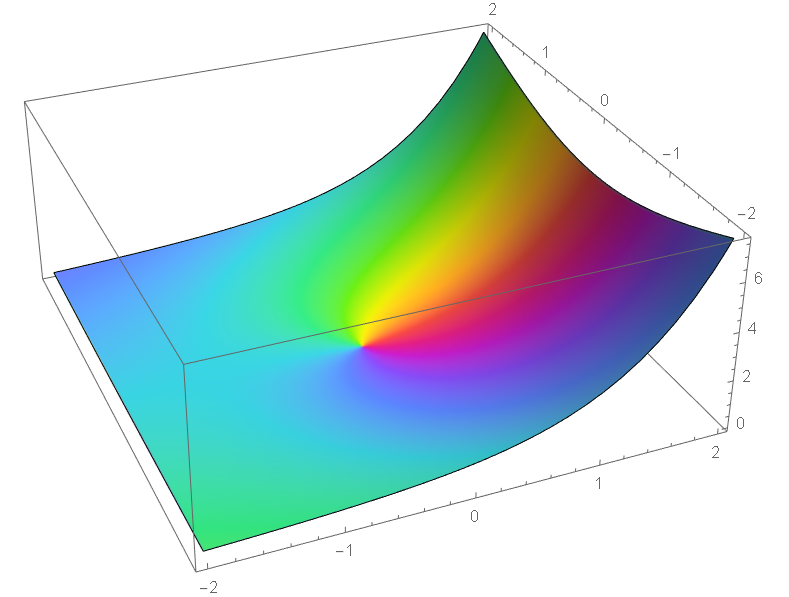
\includegraphics[width=0.75\textwidth]{4.1LHS.png}
 	 	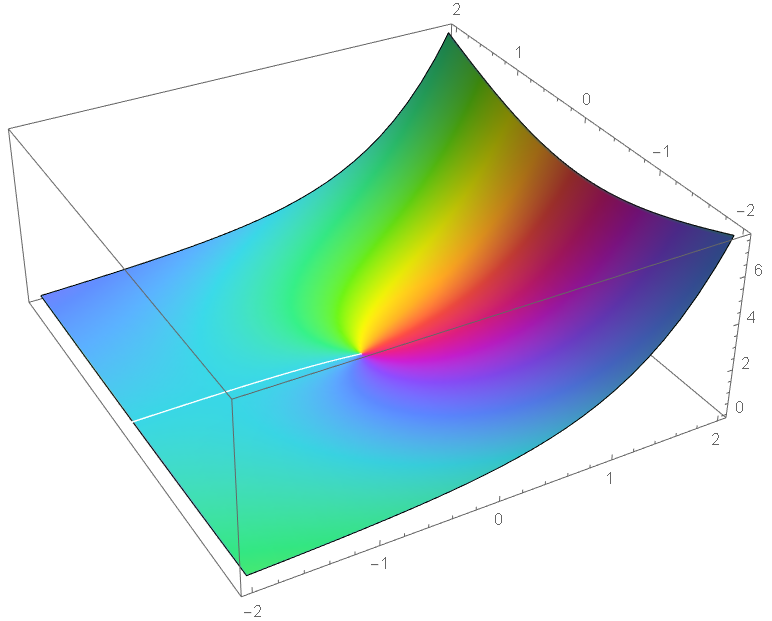
\includegraphics[width=0.75\textwidth]{4.1RHS.png}
 	\caption{The complex plot of the theorem \eqref{4.1} for $n = 2$. (Top) The left-hand side of equality. (Bottom) The right-hand side of the equality. For both plots, the $x$-axis refers to the real-part, the $y$-axis define as the imaginary part, the $z$-axis is the absolute value of the expression $\mathrm{Abs}(f)$, and the color refers to the argument of the expression $\mathrm{Arg}(f)$. Both figures generated using Wolfram Mathematica v12.1.}
 	\label{F4.1}
 \end{figure}

\noindent For accuracy check, we plot the equation of the theorem for $n=2$ into the complex plane. The plot for both sides of the equation is in Figure \ref{F4.1}. We can see that the two figures are almost identical, and we observe a visible branch cut in the figure of the right-hand side. Take note that Mathematica numerically evaluate each functions and terms individually. Thus, the appearance of branch cut is due to the of numerical artifacts of the logarithmic function $\log (z)$ and the incomplete gamma function \cite{incgamma2}
\begin{equation}
\begin{split} \label{IG}
    \Gamma(-n,\,z) = & \frac{(-1)^{n-1}}{n!} \left[ \mathrm{Ei}(-z) - \frac{1}{2} \left( \log(-z) - \log \left( \frac{-1}{z} \right) \right) + \log(z) \right] \\& \hspace{5mm} - e^{-z} \sum_{k=1}^{n} \frac{z^{k-n-1}}{(-n)_k},
\end{split}
\end{equation}
found in the right-hand side of the equation. We can see that both terms have an opposite sign and a branch cut on the same interval. This will make the branch cut to cancel each other and prove the consistency of the complex plot. Finally, the complex plot confirms the accuracy of the established theorem.

Another accuracy check is the simplification of the obtained reduction formula into some known special values. The reduction formula of the Kampé de Fériet Function in Theorem \ref{4.1} is found to be related to the hypergeometric function ${}_2F_2$  \cite[p. 3013, Eq. 3.2a]{miller2006summations}
\begin{equation}
\begin{split}
     F^{-:\;1;\;2}_{1:\;-;\;1}\left[\begin{array}{ccc}
     -:& 1; & 1, n  \\
     2:& -; & n+1 
    \end{array};\;  z,z\right]  = e^z \pFq{2}{2}{1,1}{2,n+1}{-z}.
\end{split}
\end{equation}
Thus, we can extract from the Theorem \ref{4.1} the expression:
\begin{corollary}
For complex number $z$ and positive integer $n$ the hypergeometric function ${}_2F_2$ holds the equality
\begin{equation}
\begin{split}
    \pFq{2}{2}{1,1}{2,n+1}{-z} = & \frac{n}{z} \Bigg[\mathrm{Log}(z) -\psi(n) - \frac{\Gamma(n)}{(-1)^{n}} \Gamma(1-n,\,z) \\& \hspace{20mm} + \frac{\Gamma(n)}{(-z)^{n-1}} \sum_{k=0}^{n-2} \frac{(-z)^{k}}{k!(n-1-k)} \Bigg].
\end{split}
\end{equation}
where all the functions is taken as their principal value.
\end{corollary}

The above expression was tabulated in Wolfram Function site \cite{wolfram2F2} for the cases from $n=1$ up to $n=5$. To confirm the accuracy of the Theorem \ref{4.1}, we need to reproduce the tabulated results. First, let us try for $n=1$, the above equation will give us
\begin{equation}
\begin{split} \label{n1}
    \pFq{2}{2}{1,1}{2,2}{-z} = & \frac{1}{z} \Bigg[\log(z) -\psi(1) + \Gamma(0,\,z) \Bigg].
\end{split}
\end{equation}
Using the fact that $\psi(1) = -\gamma$ where $\gamma$ is the Euler-Mascheroni constant, and the incomplete gamma function $\Gamma(0,\,z)$ \cite{incgamma} is found to be 
\begin{equation}
    \Gamma(0,\,z) = -\mathrm{Ei}(-z) + \frac{1}{2} \left( \log(-z) - \log \left( -\frac{1}{z} \right) \right) - \log(z),
\end{equation}
where $\mathrm{Ei}$ is an exponential integral. Equation \eqref{n1} will reduce to 
\begin{equation}
    \pFq{2}{2}{1,1}{2,2}{-z} =  \frac{1}{2z} \Bigg[2\gamma - 2\mathrm{Ei}(-z) +  \log(-z) - \log \left( -\frac{1}{z} \right) \Bigg].
\end{equation}
The above equation reproduce the hypergeometric function ${}_2F_2(1,1;2,2;z)$ listed in \cite{2f21}. The rest of the tabulated result can be reproduce using the recurrence relation of the digamma function \cite[Eq.~5.5.2]{NIST:DLMF} express as
\begin{equation} 
    \psi(n+1) = \psi(n) + \frac{1}{n},
\end{equation}
and the incomplete gamma function express in equation \eqref{IG}.


\section{Reduction formula from integral representation of Gauss hypergeometric function ${}_2F_1$}

In \cite{saxena1959study}, we can find a more general form of the Stietljes transform evaluated in Chapter \ref{ch_3}. The Stieltjes transform is known to be proportional to the Gauss hypergeometric function,
\begin{equation}
\int_0^{\infty} \frac{x^{\nu-1} (a+x)^{-\mu}}{(b+x)^{\rho}} \, \mathrm{d}x = \frac{\Gamma(\nu) \Gamma(\mu-\nu+\rho)}{\Gamma(\mu+\rho)} \frac{b^{\nu-\rho}}{a^{\mu}}\, \pFq{2}{1}{\mu,\nu}{\mu+\rho}{1-\frac{b}{a}},
\label{STGHF2}
\end{equation}
for $|\mathrm{Arg} \, b|<\pi$, $\mathrm{Re} (\rho+\mu-\nu)>0$. From Chapter \ref{ch_3}, we see how the summation of the digamma function arises in finite-part integral calculation specifically for the pole singularity case. Therefore, we can expect that the summation will appear for the cases where $\nu$ and $\rho$ are integers and $\nu$ and $\rho$ are non-integers with an integer difference. We will exploit the proportionality above to obtain a reduction formula of the Kampé de Fériet function.  

\subsection{Case 1: $\nu$, $\rho \in \mathbb{Z}^{+}$}

In this case, we will consider $\mu$ as any positive real number since we will choose the singularity of $f(z)$ to be located far away or $|a| > |b|$. Thus, the nature of singularity of $(a+z)^{-\mu}$ will not matter. Additionally, we will let $n = \rho$ and $m = \nu$ to be easily identified as a positive integer, $n, m \in \mathbb{Z}^{+}$. Under these conditions, the divergence will induce by the pole singularity. Therefore, we will use Theorem \ref{T3.1} to construct the finite-part integral. Implementing Theorem \ref{T3.3}, the Stieltjes transform of $(a+x)^{-\mu}$ is evaluated to be 
\begin{equation}
\begin{split}
\int_0^{\infty} \frac{x^{m-1} (a+x)^{-\mu}}{(b+x)^{n}} \, \mathrm{d}x =& \sum_{k=0}^{\infty} \, {- n \choose k} \, b^{k} \,\bbint{0}{\infty} \frac{(a+x)^{-\mu}}{x^{k+n-m+1}} \,\mathrm{d}x \\
& - \mathrm{Res} \left[ \frac{z^{m-1} \, (a+z)^{-\mu}}{(b+z)^{n}}\, \log(-z)\right]_{z=-b}.
\end{split} \label{mlessn}
\end{equation}
However, the above equality will only hold when $m < n$. Notice that the terms of the summation when $m \geq n$, the finite-part integral of the terms $0 \leq k \leq m-n-1$ is just a convergent integral. Recall the remarks in \cite{doi:10.1063/5.0038274}, the finite-part integral of a convergent integral is the value of convergent integral itself. Therefore, for $m \geq n$, the Stieltjes transform is
\begin{equation}
\begin{split} \label{mgeqn}
\int_0^{\infty} \frac{x^{m-1} (a+x)^{-\mu}}{(b+x)^{n}} \, \mathrm{d}x =& \sum_{k=0}^{m-n-1} \, {- n \choose k} \, b^{k}   \int_0^{\infty} \frac{(a+x)^{-\mu}}{x^{k+n-m+1}} \,\mathrm{d}x \\& + \sum_{k=m-n}^{\infty} \, {- n \choose k} \, b^{k} \,\bbint{0}{\infty} \frac{(a+x)^{-\mu}}{x^{k+n-m+1}} \,\mathrm{d}x \\
& - \mathrm{Res} \left[ \frac{z^{m-1} \, (a+z)^{-\mu}}{(b+z)^{n}}\, \log(-z)\right]_{z=-b}.
\end{split}
\end{equation}

The first term of the right-hand side of the equation is a convergent integral. It can evaluate easily using the integral representation of the Beta function given by equation
\begin{equation}
\int_0^{\infty} \frac{x^{d-1}}{(1+c x)^{\sigma}}\,\mathrm{d}x = c^{-d} B(d,\sigma-d),\;\; |\mathrm{arg}\,c|<\pi , \;\; \mathrm{Re}\, \sigma > \mathrm{Re}\, d>0,
\end{equation}
where $B(a,b)=\Gamma(a)\Gamma(b)/\Gamma(a+b)$ is the beta function. Applying it to our integral and doing some algebraic manipulation, we obtain the result
\begin{equation}
\int_0^{\infty} \frac{(a+x)^{-\mu}}{ x^{k+n-m+1}} \,\mathrm{d}x
= \frac{\Gamma (-k+m -n )  \Gamma (k+\mu -m +n )}{a^{k+\mu -m +n } \Gamma (\mu
   )}.
\label{BetaInt}
\end{equation}
Next, for the evaluation of the finite-part integral. we will consider the proposition below. 

\begin{proposition} \label{4.1}
Let $n, m$ be a natural number, and $a$, $\mu$ a positive real number. Then
\begin{equation}
\begin{split} \label{fp}
\bbint{0}{\infty} \frac{(a+x)^{-\mu}}{x^{k+n-m+1}}\,\mathrm{d}x = \, &\frac{1}{a^{k+n-m+\mu}} {-\mu \choose k+n-m} \\
& \hspace{-15mm} \times  \left(\log(a) + \psi(k+n-m+1) - \psi(k+n-m+\mu)\right)
\end{split}
\end{equation}
where $\psi(x)$ is a digamma function.
\end{proposition}

\begin{proof}
To prove the above equality, we consider the usual integral with a limits from $\epsilon$ to $c$
\begin{equation}
    \int_{\epsilon}^{c} \frac{(a+x)^{-\mu}}{x^{k+n-m+1}}\,\mathrm{d}x.
\end{equation}
Also, we will expand the binomial $(a+x)^{-\mu}$ at the origin. The expansion is given by
\begin{equation}
    (a+x)^{-\mu} = \sum_{l=0}^{\infty} = {-\mu \choose l} \frac{x^{l}}{a^{l+\mu}},
    \label{TE}
\end{equation} 
which is uniformly convergent for $|x| < a$. The term-wise integration is valid since the function $(a+x)^{-\mu}$ is integrable along the limits of integral $[0,c]$ and well-defined within the radius of convergence of the series. The integral will result to
\begin{equation}
\int_{\epsilon}^{c} \frac{(a+x)^{-\mu}}{x^{k+\rho-m+1}} \,\mathrm{d}x =  \sum_{l=0}^{\infty} {-\mu \choose l}  \frac{1}{a^{l+\mu}} \, \int_{\epsilon}^{c} x^{l-k-n+m-1} \,\mathrm{d}x .
\label{FPIcase1}
\end{equation}
Now, we will decompose the summation into three parts based on the results of the integral. First, the interval $0 \leq l \leq k+\rho-m-1 $ where the integral will result in a negative exponent when evaluated. The integral on term $l = k +\rho -m$ will result in a logarithm. The last interval $k +\rho - m +1 \leq l \leq \infty$ will result to the positive exponent of the integral. Performing the integral and evaluating at the limit of integration will give us
\begin{align}
\begin{split}
\int_{\epsilon}^{c} & \frac{(a+x)^{-\mu}}{x^{k+\rho-m+1}}  \, \mathrm{d}x  =  \\& \quad \sum_{l=0}^{k+\rho-m-1} \frac{{-\mu \choose l}}{a^{l+\mu}} \, \frac{1}{l-k-n+m} \, \left( \frac{1}{c^{-l+k+\rho-m}} - \frac{1}{\epsilon^{-l+k+\rho-m}} \right) \\& + \frac{{-\mu \choose k+\rho-m}}{a^{k+n+\mu-m}} \left( \ln{c} - \ln{\epsilon} \right) \\& + \sum_{l=k+n-m+1}^{\infty} \frac{{-\mu \choose l}}{a^{l+\mu}} \, \frac{1}{l-k-n+m} \, \left( c^{l-k-n+m}-\epsilon^{l-k-n+m} \right).
\label{FPIc1}
\end{split}
\end{align}
Next, we will group the terms into two based on its behavior when we take the limit $\epsilon \to 0$. The diverging terms and the converging terms are determined as follows:
\begin{align}
\begin{split}
C_{\epsilon} = \,& \sum_{l=0}^{k+n-m-1} \frac{{-\mu \choose l}}{a^{l+\mu}} \, \frac{1}{l-k-n+m}  \, \frac{1}{c^{-l+k+n-m}} + \frac{{-\mu \choose k+n-m}}{a^{l+k+n+\mu-m}} \, \ln{c} \\& + \sum_{l=k+n-m+1}^{\infty} \frac{{-\mu \choose l}}{a^{l+\mu}} \, \frac{1}{l-k-n+m}  \, \left( c^{l-k-n+m}-\epsilon^{l-k-n+m} \right)
\end{split}
\end{align}

\begin{equation}
D_{\epsilon} = \frac{{-\mu \choose k+n-m}}{a^{k+n+\mu-m}} \, \ln{\epsilon} + \sum_{l=0}^{k+n-m-1} \frac{{-\mu \choose l}}{a^{l+\mu}} \, \frac{1}{l-k-n+m}  \, \frac{1}{\epsilon^{-l+k+n-m}}
\end{equation}
By dropping the divergent terms $D_{\epsilon}$, we will obtain the finite-part integral of the equation \eqref{FPIcase1} and that is
\begin{align}
\begin{split}
\bbint{0}{c} \frac{(a+x)^{-\mu}}{x^{k+n-m+1}}  \,\mathrm{d}x \,&  =  \sum_{l=0}^{k+n-m-1} \frac{{-\mu \choose l}}{a^{l+\mu}} \, \frac{1}{l-k-n+m}  \, \frac{1}{c^{-l+k+n-m}} \\& + \frac{{-\mu \choose k+n-m}}{a^{k+n+\mu-m}} \, \ln{c} \\& + \sum_{l=k+n-m+1}^{\infty} \frac{{-\mu \choose l}}{a^{l+\mu}} \, \frac{1}{l-k-n+m}  \, c^{l-k-n+m}.
\end{split}
\end{align}
Moreover, by taking $c \to \infty$, some of the terms in the converging group will be negligible since $\frac{1}{c} \to 0 $. This action will leave us the expression
\begin{align}
\begin{split}
\bbint{0}{\infty} \frac{(a+x)^{-\mu}}{x^{k+n-m+1}} \,& \mathrm{d}x = \lim_{c \to \infty} \Bigg[  \frac{{-\mu \choose k+n-m}}{a^{k+n+\mu-m}} \, \ln{c} \\& + \sum_{l=k+n-m+1}^{\infty} \frac{{-\mu \choose l}}{a^{l+\mu}} \, \frac{1}{l-k-n+m}  \, c^{l-k-n+m} \Bigg].
\label{FPIc1v2}
\end{split}
\end{align}
To facilitate the calculation of limit and further simplify the finite-part integral, the second term of the right-hand side will be converted into the form of hypergeometric function written in equation \eqref{GHF},
\begin{align}
\begin{split}
\sum_{l=k+n-m+1}^{\infty} \frac{{-\mu \choose l}}{a^{l+\mu}} \, \frac{c^{l-k-n+m}}{l-k-n+m} \,&  = \frac{-c}{a^{k+n+\mu-m}} {-\mu \choose k+n-m}  \\&  \hspace{-10 mm} \times \pFq{3}{2}{1,1,k+n+\mu-m+1}{k+n-m+2,2}{-\frac{c}{a}}.
\end{split}
\end{align} 
Closing the series into the form of hypergeometric function serves as the analytic continuation of infinite series outside of its radius of convergence. Now, we can use the asymptotic expansion of the hypergeometric function $_3F_2$ for the case of a double pole with a large argument from equation \eqref{3F2doublepole}. Implementing the equation, the second term of the equation \eqref{FPIc1v2} reduces to
\begin{align}
\begin{split}
\,&   \frac{c}{a^{k+n+\mu-m}} {-\mu \choose k+n-m}  \pFq{3}{2}{1,1,k+n+\mu-m+1}{k+n-m+2,2}{-\frac{c}{a}} \\& \quad \quad =  \frac{\Gamma(k+n-m+2) \Gamma^2(m-k-n-\mu)} {\Gamma(1-\mu) \Gamma(1-k-n+m-\mu)} \frac{c^{m-k-n-\mu}}{a}  + \frac{{-\mu \choose k+n-m}}{a^{k+n+\mu-m}} \\& \quad \quad \quad \times \left(\log\left(\frac{c}{a}\right) + \psi(k+n+\mu-m)-\psi(k+n-m+1) \right)
\label{3f2dp}
\end{split}
\end{align}
Then, we will substitute back equation \eqref{3f2dp} back to equation \eqref{FPIc1v2}
\begin{align}
\begin{split}
& \bbint{0}{\infty} \frac{(a+x)^{-\mu}}{x^{k+n-m+1}} \, \mathrm{d}x =  \lim_{c \to \infty} \ \Bigg[  \frac{{-\mu \choose k+n-m} \ln{c}}{a^{k+n+\mu-m}} \\& \hspace{20mm} - \frac{\Gamma(k+n-m+2) \Gamma^2(m-k-n-\mu)} {\Gamma(1-\mu) \Gamma(1-k-n+m-\mu)}   \frac{c^{m-k-n-\mu}}{a} \\&  - \frac{{-\mu \choose k+n-m}}{a^{k+n+\mu-m}}  \left(\ln\left(\frac{c}{a}\right)  + \psi(k+n+\mu-m)-\psi(k+n-m+1) \right) \Bigg].
\label{5.26}
\end{split}
\end{align}
Performing the limit will make the second term in the right-hand side of the equation vanish since the exponent of $c$ in that terms is negative. Also, the two terms with the logarithm will cancel each other. Thus, we evaluated the finite-part integral to be
\begin{align}
\begin{split}
\bbint{0}{\infty} \frac{(a+x)^{-\mu}}{x^{k+n-m+1}} \,& \mathrm{d}x = \frac{{-\mu \choose k+n-m}}{a^{k+n+\mu-m}} \\& \times \left(\ln(a) + \psi(k+n-m+1) - \psi(k+n+\mu-m) \right).
\label{FPI1final}
\end{split}
\end{align}
\end{proof}

Lastly, for the evaluation of the residue. This residue can be evaluated using its differentiation form written as
\begin{equation}
    \mathrm{Res}(f, c) = \frac{1}{(n-1)!} \lim_{z \to c} \, \frac{\mathrm{d}^{n-1}}{\mathrm{d}z^{n-1}} \, ((z-c)^{n} f(z)),
    \label{5.28}
\end{equation}
where $c$ is the pole with order $n$. We will use the General Leibniz rule to evaluate this differentiation. The general Leibniz rule is the generalization of the product rule, which states that if $f$ and $g$ are n-times differentiable, then its product $fg$ will also n-times differentiable. The $n$th derivatives of the function $fg$ is written as
\begin{equation}
    (fg)^{(n)} =  \sum_{k=0}^{n} {n \choose k} \, f^{(n-k)} g^{(k)}
\end{equation}
where ${n \choose k} = \frac{n!}{k!(n-k)!}$ is the binomial coefficient. This can be proved using product rule and mathematical induction. Expressing the residue in equation \eqref{5.28} in its differentiation form will give us
\begin{align}
\begin{split}
    \mathrm{Res} \,& \left[\frac{z^{m-1} \, (a+z)^{-\mu}}{(b+z)^{n}}\, \log(-z) \right]_{z=-b} \\& = \frac{1}{(n-1)!} \lim_{z \to -b} \, \frac{\mathrm{d}^{n-1}}{\mathrm{d}z^{n-1}} \, ( z^{m-1 }(a+z)^{-\mu} \log(-z)).
\end{split}
\end{align}
In applying the General Leibniz rule, we will choose $f(z) =  (a+z)^{-\mu}$ and $g(z) = z^{m-1} \log(-z)$, rewriting the above residue
\begin{align}
\begin{split}
   & \mathrm{Res}  \left[\frac{z^{m-1} \, (a+z)^{-\mu}}{(b+z)^{n}}\, \log(-z) \right]_{z=-b} \\& = \frac{1}{(n-1)!} \lim_{z \to -b} \, \sum_{k=1}^{n-1} {n -1 \choose k} \, \frac{\mathrm{d}^{n-1-k}}{\mathrm{d}z^{n-1-k}} (a+z)^{-\mu} \, \frac{\mathrm{d}^{k}}{\mathrm{d}z^{k}}  (z^{m-1 } \log(-z)).
    \label{5.31}
\end{split}
\end{align}
Now, evaluate the $(n-1-k)$th derivative of $(a+z)^{-\mu}$
\begin{equation}
    \frac{\mathrm{d}^{n-1-k}}{\mathrm{d}z^{n-1-k}} (a+z)^{-\mu}= (k-\mu-n+2)_{n-1-k} \, (a+z)^{k-\mu-n+1}.
    \label{5.32}
\end{equation}
For the other differentiation, since it is a product of two function, we will use again the general Leibniz rule where we consider $h(z)=z^{m-1}$ and $i(z) = \log(-z)$. The differentiation can be written as 
\begin{equation}
    \frac{\mathrm{d}^{k}}{\mathrm{d}z^{k}} ( z^{m-1 }\log(-z)) = \sum_{l=0}^{k} {k \choose l} \,  \frac{\mathrm{d}^{k-l}}{\mathrm{d}z^{k-l}} (z^{m-1})  \frac{\mathrm{d}^{l}}{\mathrm{d}z^{l}} \log(-z).
    \label{5.33}
\end{equation}
Evaluating the derivatives, we obtain
\begin{equation}
     \frac{\mathrm{d}^{k-l}}{\mathrm{d}z^{k-l}} (z^{m-1}) = \frac{(m+l-k)_{k-l}}{z^{k-l-m+1}}
     \label{5.34}
\end{equation}
and
\begin{equation}
     \frac{\mathrm{d}^{l}}{\mathrm{d}z^{l}} \log(-z) =  \begin{cases} 
      \log(-z) & l = 0 \\
      -\frac{\Gamma(l)}{(-z)^{l}} & otherwise
   \end{cases}.
     \label{5.35}
\end{equation}
Combining the result in equation \eqref{5.34} and equation \eqref{5.35}, the equation \eqref{5.33} is evaluated as

\begin{align}
\begin{split}
\frac{\mathrm{d}^{k}}{\mathrm{d}z^{k}} ( z^{m-1 }\log(-z)) = \frac{\Gamma(m)}{\Gamma(k-m)} \frac{\log(-z)}{z^{k-m+1}} +\sum_{l=1}^{k} {k \choose l} \,  \frac{\Gamma(m) \, \Gamma(l)}{\Gamma(l-m+k)} \frac{(-1)^{l+1}}{z^{k-m+1}}.
\label{5.36}
\end{split}
\end{align}
To completely evaluate the residue, we substitute back equation \eqref{5.32} and equation \eqref{5.36} back to the residue equation \eqref{5.31}, taking the limit of $z \to -b$ and simplifying it gives us
\begin{align}
\begin{split}
    &\mathrm{Res} \left[\frac{z^{m-1} \, (a+z)^{-\mu}}{(b+z)^{n}}\, \log(-z) \right]_{z=-b} \\& \quad = \frac{1}{(n-1)!} \sum_{k=1}^{n-1} {n -1 \choose k} \, (k-\mu-n+2)_{n-1-k} \, (a-b)^{k-\mu-n+1} \\& \quad \times \left( (m-k)_{k} \frac{\ln(b)}{(-b)^{k-m+1}} + \sum_{l=1}^{k} {k \choose l} (m-k+l)_{k-l} \frac{\Gamma(l)  (-1)^{l-1}}{(-b)^{k-m+1}}  \right).
    \label{residue}
\end{split}
\end{align}
Since $m$ is a positive integer, it is clear that the expression for the residue term depends on the relative values of $m$ and $n$. We see that all terms involve is also dependent on the value of $m$ and $n$. Hence, we will consider them separately. 

\subsubsection{Case $m > n$}In this case, implementing the method will result in equation \eqref{mgeqn}. The results are composed of convergent integral, a term containing the finite-part integral, and a residue. The convergent integral is evaluated using the integral representation of beta function found in equation \eqref{BetaInt}. Substituting this integral back into the series will result to
\begin{equation}
\begin{split} \label{CI5.3}
&\sum_{k=0}^{m-n-1} \, {- n \choose k} \, b^{k}   \int_0^{\infty} \frac{(a+x)^{-\mu}}{x^{k+n-m+1}} \,\mathrm{d}x = \frac{b^{m-n}}{a^{\mu}} \left(\frac{a}{b}\right)^{m-n} (\mu)_{n-m}\\
&\hspace{12mm}\times\sum_{k=0}^{m-n-1} \frac{(-1)^k 
	(n)_k (\mu-m+n)_k (m-n-k-1)!}{k!} \left(\frac{b}{a}\right)^k.
 \end{split}
\end{equation} 
For the second term, an infinite series composed of finite-part integral, we can  use the preposition \ref{4.1} to evaluate the finite-part integral and perform a shift in summation. This will result to the equality
\begin{equation} \label{SFS}
	\begin{split}
	&\sum_{k=m-n}^{\infty} \, {- n \choose k} \, b^{k} \,\bbint{0}{\infty} \frac{(a+x)^{-\mu}}{x^{k+n-m+1}} \,\mathrm{d}x = \frac{b^{m-n}}{a^{\mu} }\frac{(-1)^{m-n} (m-1)!}{(n-1)! (m-n)!}\\ &\hspace{15mm}\times\sum_{k=0}^{\infty} \frac{(m)_k (\mu)_k}{(m-n+1)_k k!} \left[\ln(a)+\psi(k+1)-\psi(k+\mu)\right]\left(\frac{b}{a}\right)^k .
	\end{split}
\end{equation}
valid for $|b/a| < 1$. Lastly, for the more simplified form of the residue in equation \eqref{residue}. We will use the evaluated inner sum
\begin{equation} \label{4.22}
\sum_{l=1}^{k} (-1)^{l-1} {k \choose l} (m-k+l)_{k-l} \Gamma(l)=\frac{\Gamma (m) (\psi(m)-\psi(m-k))}{\Gamma (m-k)}
\end{equation}

Substituting these back into equation \eqref{residue} and performing some simplifications, we obtain
\begin{equation}
\begin{split}
   & \mathrm{Res} \, \left[\frac{z^{m-1} \, (a+z)^{-\mu}}{(b+z)^{n}}\, \log(-z) \right]_{z=-b} 
   \\&\hspace{4mm}= \frac{(m-1)!  (-1)^{m-n}}{a^{n-m+\mu}} \left(1-\frac{b}{a}\right)^{-\mu} 
   \sum_{l=0}^{n-1} \frac{(\mu)_l}{(n-1-l)! (m-n+l)! \,l!}  \\&\hspace{10mm}\times \left[\ln(b)+\psi(m)-\psi(m-n+1+l)\right]\left(\frac{b/a}{1-b/a}\right)^l.
    \end{split}
\end{equation}

We now gather all the terms together and substitute them back into equation \eqref{mgeqn}, we obtain
\begin{equation}\label{rawresult4a}
\begin{split}
&\frac{\Gamma(m) \Gamma(\mu-m+n)}{\Gamma(\mu+n)}\;\pFq{2}{1}{\mu,m}{\mu+n}{1-\frac{b}{a}} = \left(\frac{a}{b}\right)^{m-n} (\mu)_{n-m} \\& \hspace{15mm} \times
\sum_{k=0}^{m-n-1} \frac{(-1)^k 
	(n)_k (\mu-m+n)_k (m-n-k-1)!}{k!} \left(\frac{b}{a}\right)^k
	\\&\hspace{4mm} +\frac{(-1)^{m-n}(m-1)!}{(n-1)! (m-n)!}\sum_{k=0}^{\infty} \frac{(m)_k (\mu)_k}{(m-n+1)_k k!} \\&\hspace{15mm}\times\left[\ln(a)+\psi(k+1)-\psi(k+\mu)\right]\left(\frac{b}{a}\right)^k\\
&\hspace{4mm}-(-1)^{m-n} \left(1-\frac{b}{a}\right)^{-\mu} (m-1)! \sum_{l=0}^{n-1} \frac{(\mu)_l}{(n-1-l)! (m-n+l)! \,l!}  \\
&\hspace{15mm}\times \left[\ln(b)+\psi(m)-\psi(m-n+1+l)\right]\left(\frac{b/a}{1-b/a}\right)^l 
\end{split}
\end{equation}

The left hand side of this equation is in terms of the variable $b/a$ and so must the left hand side be. This is only possible if the coefficients of $\ln(a)$ and $\ln(b)$ are the same. To show that that is the case, we use the known transformation formula \cite[p. 64, 22]{bateman1953higher} given by
\begin{equation} \label{transform}
\pFq{2}{1}{a,b}{c}{z}=(1-z)^{-a} \pFq{2}{1}{a,c-b}{c}{\frac{z}{z-1}}
\end{equation}
which is valid for $|z|<1$ and $|z/(z-1)|<1$. We apply this on the coefficient of $\ln(a)$, which is given by
\begin{equation}
\begin{split}
\sum_{k=0}^{\infty} \frac{(m)_k (\mu)_k}{(m-n+1)_k k!} z^k &=  \pFq{2}{1}{\mu,m}{m-n+1}{z}\\
&=(1-z)^{-\mu}\pFq{2}{1}{\mu,1-n}{m-n+1}{\frac{z}{z-1}} .
\end{split}
\end{equation}
Since $n$ is a natural number, the upper parameter $(1-n)$ takes on the value equal to zero or a negative integer. The hypergeometric function in the right hand side reduces to a polynomial of order $(n-1)$. Expanding the right hand side and performing the substitutions
\begin{equation}
(1-n)_l = (-1)^l \frac{(n-1)!}{(n-1-l)!},\;\;\; (m-n+1)_l = \frac{(m-n+l)!}{(m-n)!},
\end{equation} 
we obtain the equality
\begin{equation}
\begin{split}
\frac{1}{(n-1)! (m-n)!}\sum_{l=0}^{\infty} \frac{(m)_k (\mu)_k}{(m-n+1)_k k!} z^k&\\
&\hspace{-50mm} = (1-z)^{-\mu} \sum_{k=0}^{n-1} \frac{(\mu)_l}{(n-1-l)! (m-n+l)! l!} \left(\frac{z}{1-z}\right)^l .
\end{split}
\end{equation}
The right-hand side of the equation is indeed the coefficient of $\ln{b}$. This allows us to combine the logarithmic terms in two ways. Then the entire expression of the right hand side of equation \eqref{rawresult4a} is now in terms of the variable $b/a$. By analytic continuation, we can replace this with the complex variable $z$ and simplified the expression into
	\begin{equation}\label{result4av0}
	\begin{split}
	&\frac{\Gamma(m) \Gamma(\mu-m+n)}{\Gamma(\mu+n)}\;\pFq{2}{1}{\mu,m}{\mu+n}{1-z}\\
	& = \frac{1}{z^{m-n}} (\mu)_{n-m}
	\sum_{k=0}^{m-n-1} \frac{(-1)^k 
		(n)_k (\mu-m+n)_k (m-n-k-1)!}{k!} z^k\\
	&\hspace{4mm}+\frac{(-1)^{m-n}(m-1)!}{(n-1)! (m-n)!}  \\&\hspace{10mm} \times\sum_{k=0}^{\infty} \frac{(m)_k (\mu)_k \left[-\ln(z)-\psi(m)+\psi(k+1)-\psi(k+\mu)\right]}{(m-n+1)_k k!} z^k\\
	&\hspace{4mm}+(-1)^{m-n} \left(1-z\right)^{-\mu} (m-1)!   \\&\hspace{10mm} \times \sum_{l=0}^{n-1} \frac{(\mu)_l \,\psi(m-n+1+l)}{(n-1-l)! (m-n+l)! \,l!} \left(\frac{z}{1-z}\right)^l
	\end{split}
	\end{equation}
 Using the definition of function ${}_p\tilde{\psi}_q$ found in equation \eqref{psi}, we can rewrite the equation in terms of it. The other series can also express in terms of hypergeometric function. In addition, we lift the restriction that $\mu$ is real using the same principle. Doing so, we obtain the result.

\begin{theorem} \label{result4a} Let $m$ and $n$ be positive integers with $m>n$, and $\mu$ a complex number with $(\mu-m+n)\neq 0, -1, -2, \dots$. Then
	\begin{equation}
	\begin{split}
	&\frac{\Gamma(m) \Gamma(\mu-m+n)}{\Gamma(\mu+n)}\;\pFq{2}{1}{\mu,m}{\mu+n}{1-z}\\
	& = \frac{(-1)^{\nu-\rho+1}}{z} \frac{\Gamma(\nu-1)}{(\mu-1)\Gamma(\rho)\Gamma(\nu-\rho)} \, \pFq{3}{2}{1-m-n,1,1}{2-\mu,2-m}{\frac{1}{z}} \\
	&\hspace{4mm}-\frac{(-1)^{m-n}(m-1)!}{(n-1)! (m-n)!} \, \Bigg[\pFq{2}{1}{m, \mu}{m-n+1}{z} (\mathrm{Log}(z) - \psi(m)) 
	\\&\hspace{15mm}+ \pPq{2}{1}{m,\mu}{m-n+1}{\mu}{z} - \pPq{2}{1}{m,\mu}{m-n+1}{1}{z}\Bigg]
	\\&\hspace{4mm}+\frac{(-1)^{m-n} }{\left(1-z\right)^{\mu}}  (m-1)!   \sum_{l=0}^{n-1} \frac{(\mu)_l \,\psi(m-n+1+l)}{(n-1-l)! (m-n+l)! \,l!} \left(\frac{z}{1-z}\right)^l
	\end{split}
	\end{equation}
	for $z \not =1$ and $|\mathrm{arg}(z)|<\pi$. All the functions involve are taken as their principal value. 
\end{theorem}
\noindent The above relation appears to be new identity of Gauss hypergeomteric function.

We now wish to exploit the hypergeometric-type series containing the digamma function to generate a reduction formula of the Kampé de Fériet function. By the existing relation in equation \eqref{DxK}, we can construct the following relations:
\begin{align}
\begin{split}
    \pPq{2}{1}{m,\mu}{m-n+1}{1}{z} &  = -\gamma \, \pFq{2}{1}{m,\mu}{m-n+1}{z}  \\&\hspace{-25mm}  + z\, \frac{\mu \, m}{m-n+1} \, F^{2 \, 1 \, 2}_{2 \, 0 \, 1}\left[\begin{array}{lll}
	\mu+1, m+1 &: 1 &; 1,1  \\
	2, m-n+2&:  &; 2 
	\end{array};\; z,z\right]
\end{split}
\end{align}
and
\begin{align}
\begin{split}
    \pPq{2}{1}{m,\mu}{m-n+1}{1}{z} & = \psi(\mu) \, \pFq{2}{1}{m,\mu}{m-n+1}{z}  \\&\hspace{-25mm} + z\, \frac{ \, m}{m-n+1} \, F^{2 \, 1 \, 2}_{2 \, 0 \, 1}\left[\begin{array}{lll}
	\mu+1, m+1 &: 1 &; 1,\mu  \\
	2, m-n+2&:  &; \mu+1 
	\end{array};\; z,z\right].
\end{split}
\end{align}
Now, we substitute the above relations to the Theorem \ref{result4a} and isolate the Kampé de Fériet function. This will tabulate a recurrence relation of the reduction formula of Kampé de Fériet function. Additionally, the infinite series can be expressed as a hypergeometric function using equation \eqref{GHF}.

\begin{corollary} \label{4.2.1}
Let $m$ and $n$ be positive integers with $m>n$, and $\mu$ a complex number with $(\mu-m+n)\neq 0, -1, -2, \dots$. Then
	\begin{equation}
	\begin{split} \label{e4.2.1}
    F^{2 \, 1 \, 2}_{2 \, 0 \, 1}&\left[\begin{array}{lll}
	\mu+1, m+1 &: 1 &; 1,\mu  \\
	2, m-n+2&:  &; \mu+1 
	\end{array};\; z,z\right] \\& \hspace{-10mm} - \mu \, F^{2 \, 1 \, 2}_{2 \, 0 \, 1}\left[\begin{array}{lll}
	\mu+1, m+1 &: 1 &; 1,1  \\
	2, m-n+2&:  &; 2 
	\end{array};\; z,z\right] \\& \hspace{5mm} = -\frac{(m-n)_{2}}{z^2 m^2} \pFq{3}{2}{1-m-n,1,1}{2-\mu,2-m}{\frac{1}{z}}
	\\& \hspace{10mm} -\frac{m-n+1}{z \, m} \pFq{2}{1}{m,\mu}{m-n+1}{z} 
	\\& \hspace{20mm} \times \left[ \mathrm{Log}(z) + \psi(m) + \psi(\mu) + \gamma \right] 
	\\& \hspace{10mm} -(-1)^{n-m} \frac{\Gamma(n) \Gamma(\mu-m+n)!}{z \, m \, \Gamma(\mu+n)}  \pFq{2}{1}{m,\mu}{\mu+n}{1-z} 
	\\& \hspace{10mm} -\frac{\left(1-z\right)^{-\mu}}{z \, m}  \sum_{l=0}^{n-1} \frac{(\mu)_l \,\psi(m-n+1+l)}{(n-2)_l (m-n-1)_l \,l!} \left(\frac{z}{1-z}\right)^l
	\end{split}
	\end{equation}
	for all $z \not = 1$ and $|\mathrm{arg}(z)|<\pi$.
 All the functions involve are taken as their principal values.  All the functions involve are taken as their principal value. \end{corollary}  


\begin{figure}[t]
 	\centering
 	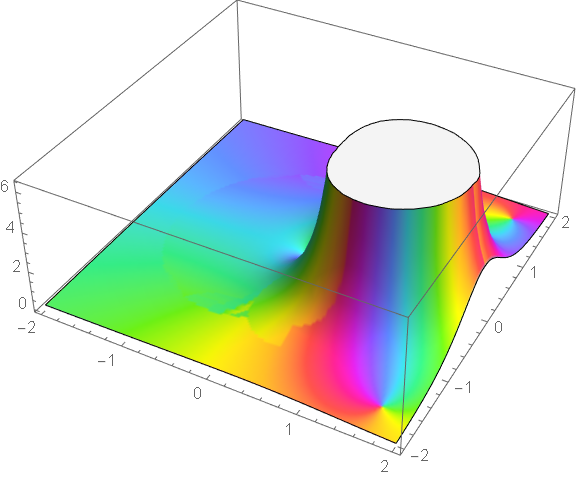
\includegraphics[width=0.75\textwidth]{4.2LHS.png}
 	 	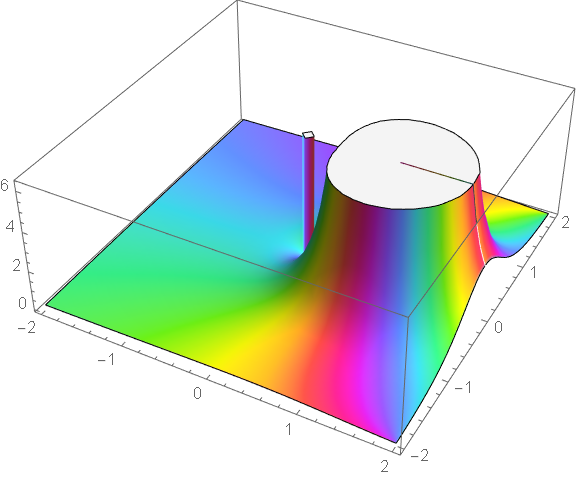
\includegraphics[width=0.75\textwidth]{4.2RHS.png}
 	\caption{The complex plot of the Corollary \ref{4.2.1} for $\mu = \pi + i$, $m=2$, and $n=1$. (Top) The left-hand side of equality. (Bottom) The right-hand side of the equality. For both plots, the $x$-axis refers to the real-part, the $y$-axis define as the imaginary part, the $z$-axis is the absolute value of the expression $\mathrm{Abs}(f)$, and the color refers to the argument of the expression $\mathrm{Arg}(f)$. Both figures generated using Wolfram Mathematica v12.1.}
 	\label{F4.2.1}
 \end{figure}

The above corollary is observe to extends the analyticity outside the region $|z|<1$. This extension is due to the analytic continuation of the function and we can verify it through the complex plot of the equality. Similar to the previous theorem, we plot the left-hand and right-hand side of the equation \eqref{e4.2.1} as a complex plot . This complex plots can be seen in Figure \ref{F4.2.1}. We can see that both plots have a singularity at $z=1$. For the difference of the two plot, we can observe that the right-hand side complex plot has a singularity at $z=0$, which come from the factor $1/z$. Also, it has a branch cut runs along the interval $[1, \infty]$ thas is induce by the hypergeometric function. The manifestation of the branch cut and pole is due to the numerical artifact since Mathematica numerically evaluate the term individually.

\subsubsection{Case $m \leq n$}

When $m \leq n$, all the integrals on the expansion are divergent, and therefore, equation \eqref{mlessn} will hold in this case. The finite part integral is already evaluated in equation \eqref{fp}. Substituting the result to the series, we will have
\begin{equation}
	\begin{split}
	&\sum_{k=0}^{\infty} \, {- n \choose k} \, b^{k} \,\bbint{0}{\infty} \frac{(a+x)^{-\mu}}{x^{k+n-m+1}} \,\mathrm{d}x \\&\hspace{8mm} =  \frac{1 }{a^{n-m+\mu} }\frac{(-1)^{n-m} (n-m+\mu-1)!}{(\mu-1)! (n-m)!} \sum_{k=0}^{\infty} \frac{(n-m+\mu)_k (n)_k}{(n-m+1)_k k!} \\& \hspace{15mm} \times \left[\ln(a)+\psi(k+n-m+1)-\psi(k+n-m+\mu)\right]\left(\frac{b}{a}\right)^k.
	\end{split}
\end{equation}
This is valid for $b/a<1$. Now, we can summed the logarithmic term as a hypergeometric function. This result to
\begin{equation}
\begin{split}
&\sum_{k=0}^{\infty} \, {- n \choose k} \, b^{k} \,\bbint{0}{\infty} \frac{(a+x)^{-\mu}}{x^{k+n-m+1}} \,\mathrm{d}x = \frac{1 }{a^{n-m+\mu} }\frac{(-1)^{n-m} (n-m+\mu-1)!}{(\mu-1)! (n-m)!}\\ &\hspace{4mm}\times\Bigg[\pFq{2}{1}{n-m+\mu,n}{n-m+1}{\frac{b}{a}}\ln(a)  +\sum_{k=0}^{\infty} \frac{(n-m+\mu)_k (n)_k}{(n-m+1)_k k!} \\ &\hspace{16mm} \times [\psi(k+n-m+1)  -\psi(k+m-n+\mu)]\left(\frac{b}{a}\right)^k\Bigg].
\end{split}
\end{equation}
Lastly, for the evaluation of residue, we will use equation \eqref{residue}. Since $n > m$, the term with logarithm for $l = m ,1, ... , n-1$ will just give a zero distribution because of the factor $1/\Gamma(m-k)$
\begin{equation}
\begin{split} 
&\mathrm{Res}  \left[ \frac{z^{m-1} \, (a+z)^{-\mu}}{(b+z)^{n}} \, \log(-z) \right]_{z=-b} 
\\& = \frac{1}{(n-1)!} \sum_{k=0}^{m-1} {n-1 \choose k} \frac{(a-b)^{k-\mu-n+1}}{(-b)^{k-m+1}} \\&\hspace{12mm} \times \frac{\Gamma(1-\mu)}{\Gamma(k-\mu-n+2)}  \frac{\Gamma(m) }{\Gamma(m-k)} \ln(b)  \\& + \frac{1}{(n-1)!} \sum_{k=1}^{n-1} {n -1 \choose k} \, (k-\mu-n+2)_{n-1-k} \, (a-b)^{k-\mu-n+1}\\&\hspace{12mm} \times \sum_{l=1}^{k} {k \choose l} (m-k+l)_{k-l} \frac{\Gamma(l)  (-1)^{l-1}}{(-b)^{k-m+1}}  .
\end{split}
\end{equation}
 Performing some more simplification. we will obtain
\begin{equation}
\begin{split}
   & \mathrm{Res} \, \left[\frac{z^{m-1} \, (a+z)^{-\mu}}{(b+z)^{n}}\, \log(-z) \right]_{z=-b} 
   \\&\hspace{4mm} = \frac{(-1)^{n-m}}{a^{n-m+\mu}} \left(1-b/a\right)^{m-n-\mu} \frac{(n-m+\mu)!(m-1)!}{(\mu-1)!} \\&\hspace{10mm}\times \sum_{l=0}^{m-1}   \frac{(n-m+\mu)_l \ln(b)}{(m-l-1)! (l+n-m)! \,l!} \left(\frac{b/a}{1-b/a}\right)^l
   \\&\hspace{5mm} + \Gamma(m)\Gamma(1-\mu) \sum_{k=1}^{n-1} \sum_{l=1}^{k}  \frac{\Gamma(k-l+1)(-1)^{k-l-m}}{(l)_{1}\Gamma(m-k+l) \Gamma(k-n-\mu+2)  }\\&\hspace{10mm}\times \left( 1-\frac{b}{a} \right)^{k-\mu-n+1} \frac{a^{k-\mu-n+1}}{b^{k-m+1}}.
    \label{residue2}
\end{split}
\end{equation}
Now, gathering all the terms together and substitute them back into equation \eqref{mlessn}, we obtain
\begin{equation}\label{rawresult4b}
\begin{split}
&\frac{\Gamma(m) \Gamma(\mu-m+n)}{\Gamma(\mu+n)}\;\pFq{2}{1}{\mu,m}{\mu+n}{1-\frac{b}{a}}\\
&\hspace{4mm} = \left(\frac{-b}{a}\right)^{n-m} \frac{(n-m+\mu-1)!}{(\mu-1)! (n-m)!}\times\Bigg[\pFq{2}{1}{n-m+\mu,n}{n-m+1}{\frac{b}{a}}\ln(a)  \\ &\hspace{8mm} +\sum_{k=0}^{\infty} \frac{(n-m+\mu)_k (n)_k}{(n-m+1)_k k!} [\psi(k+n-m+1)-\psi(k+n-m+\mu)]\left(\frac{b}{a}\right)^k\Bigg]
\\&\hspace{4mm}- \left(\frac{-b}{a}\right)^{n-m} \left(1-b/a\right)^{m-n-\mu} \frac{(n-m+\mu-1)!(m-1)!}{(\mu-1)!}  \\
   &\hspace{12mm}\times \sum_{l=0}^{m-1} \frac{(n-m+\mu)_l \ln(b)}{(m-l-1)! (l+n-m)! \,l!} \left(\frac{b/a}{1-b/a}\right)^l 
   \\&\hspace{4mm}+ \Gamma(m)\Gamma(1-\mu) \sum_{k=1}^{n-1} \sum_{l=1}^{k}  \frac{\Gamma(k-l+1)(-1)^{k-l-m}}{(l)_{1}\Gamma(m-k+l) \Gamma(k-n-\mu+2)  }
   \\&\hspace{12mm}\times \left( 1-\frac{b}{a} \right)^{k-\mu-n+1} \left( \frac{a}{b}\right)^{k-n+1}.
\end{split}
\end{equation}

Similar to the previous case, we need to show that the coefficient of the logarithm is negative of each other. This will allow as to combine the terms and make the variable all in terms of $b/a$. Starting with the transform from equation \eqref{transform} and applying it to the coefficient of $\ln({a})$, we will have
\begin{equation}
\begin{split}
\sum_{k=0}^{\infty} \frac{(n-m+\mu)_k (n)_k}{(n-m+1)_k k!} z^k &=  \pFq{2}{1}{n-m+\mu,n}{n-m+1}{z}\\
&=(1-z)^{m-n-\mu}\\& \hspace{10mm} \times\pFq{2}{1}{n-m+\mu,1-m}{n-m+1}{\frac{z}{z-1}} .
\end{split}
\end{equation}
Doing the same process from the previous case, the upper parameter $(1-m)$ takes on the value equal to zero or a negative integer. The hypergeometric function in the right-hand side reduces to a polynomial of order $(m-1)$. Expanding and performing the substitutions
\begin{equation}
(1-m)_l = \frac{(-1)^{l}(m-1)!}{(m-l-1)!},\;\;\; (n-m+1)_l = \frac{(l+n-m)!}{(n-m)!}
\end{equation} 
We obtain the equality
\begin{equation}
\begin{split}
&\frac{(n-m+\mu-1)!}{(\mu-1)! (n-m)!} (-1)^{n-m} \sum_{k=0}^{\infty} \frac{(n-m+\mu)_k (n)_k}{(n-m+1)_k k!} z^k \\
&\hspace{4mm} = (1-z)^{m-n-\mu} \frac{(m-1)!(-\mu)!}{(m-n-\mu)!}  \sum_{k=0}^{m-1} \frac{(n-m+\mu)_l}{ (m-l-1)!(l+n-m)! l!} \left(\frac{z}{1-z}\right)^l .
\end{split}
\end{equation}
This allows us to combine the logarithmic terms and by analytic continuation we can replace $b/a$ with the complex variable z. Also, we now lift the restriction that $\mu$ is real. Similar to the previous case, we will rewrite the other infinite series in terms of the function ${}_p\tilde{\psi}_q$ using its definition from equation \eqref{psi}. We obtain the result.
\begin{theorem} \label{4.3}
Let $m$ and $n$ be positive integers with $m<n$, and $\mu$ a complex number with $(\mu-m+n)\neq 0, -1, -2, \dots$. Then
\begin{equation}\label{result4b}
\begin{split}
&\frac{\Gamma(m) \Gamma(\mu-m+n)}{\Gamma(\mu+n)}\;\pFq{2}{1}{\mu,m}{\mu+n}{1-z}\\
&\hspace{4mm} = \left(-z\right)^{n-m} \frac{(n-m+\mu-1)!}{(\mu-1)! (n-m)!} \Bigg[ \pFq{2}{1}{n-m+\mu,n}{n-m+1}{z} \mathrm{Log}(z) \\ 
&\hspace{35mm}  + \pPq{2}{1}{n-m+\mu,n}{n-m+1}{n-m+1}{z}  \\ 
&\hspace{40mm} -\pPq{2}{1}{n-m+\mu,n}{n-m+1}{n-m+\mu}{z} \Bigg]
   \\&\hspace{4mm}+ \sum_{k=1}^{n-1} \sum_{l=1}^{k}  \frac{\Gamma(m)\Gamma(1-\mu)\Gamma(k-l+1)(-1)^{k-l-m}}{z^{-\mu}(l)_{1}\Gamma(m-k+l) \Gamma(k-n-\mu+2)}  \left( \frac{1-z}{z} \right)^{k-\mu-n+1}.
\end{split}
\end{equation}
for all $z\not=1$ and $|\mathrm{arg}(z)|<\pi$. All the functions involve are taken as their principal value. 
\end{theorem}
\noindent The above equality looks like a new identity of the Gauss hypergeometric function.

Similar to the previous case, we will now exploit the hypergeometric-type series containing the digamma function to generate a reduction formula of the Kampé de Fériet function. Using the relation in equation \eqref{DxK}, we can construct the following relations:
\begin{align}
\begin{split}
    \pPq{2}{1}{n-m+\mu,n}{n-m+1}{n-m+1}{z} &\\&\hspace{-50mm} =  \psi(n-m+1) \, \pFq{2}{1}{n-m+\mu,n}{n-m+1}{z} + z\, \frac{(n-m+\mu) \, n}{n-m+1} \\& \hspace{-45mm} \times  F^{2 \, 1 \, 2}_{2 \, 0 \, 1}\left[\begin{array}{lll}
	n-m+\mu+1, n+1 &: 1 &; 1,n-m+1  \\
	2, n-m+2&:  &; n-m+2 
	\end{array};\; z,z\right]
\end{split}
\end{align}
and
\begin{align}
\begin{split}
    \pPq{2}{1}{n-m+\mu,n}{n-m+1}{n-m+\mu}{z} &\\&\hspace{-50mm} = \psi(n-m+\mu) \, \pFq{2}{1}{n-m+\mu,n}{n-m+1}{z}  + z\, \frac{ \, n}{n-m+1} \\& \hspace{-45mm} \times F^{2 \, 1 \, 2}_{2 \, 0 \, 1}\left[\begin{array}{lll}
	n-m+\mu+1, n+1 &: 1 &; 1,n-m+\mu  \\
	2, n-m+2&:  &; n-m+\mu+1 
	\end{array};\; z,z\right].
\end{split}
\end{align}

Using the above relation and expressing the infinite series as a hypergeometric function, we will obtain a corollary of theorem \ref{4.3}. 

\begin{corollary} \label{4.3.1e}
Let $m$ and $n$ be positive integers with $m>n$, and $\mu$ a complex number with $(\mu-m+n)\neq 0, -1, -2, \dots$. Then
	\begin{equation}
	\begin{split}\label{4.3.1}
    F^{2 \, 1 \, 2}_{2 \, 0 \, 1}&\left[\begin{array}{lll}
	n-m+\mu+1, n+1 &: 1 &; 1,n-m+\mu  \\
	2, n-m+2&:  &; n-m+\mu+1 
	\end{array};\; z,z\right] \\& \hspace{-10mm} - (n-m+\mu) \, F^{2 \, 1 \, 2}_{2 \, 0 \, 1}\left[\begin{array}{lll}
	n-m+\mu+1, n+1 &: 1 &; 1,n-m+1  \\
	2, n-m+2&:  &; n-m+2 
	\end{array};\; z,z\right] \\& \hspace{5mm} =
	 \frac{n-m+1}{z \, n} \pFq{2}{1}{n-m+\mu,n}{n-m+1}{z} 
	\\& \hspace{15mm} \times \left[ \psi(n-m+1) -\psi(n-m+\mu) - \mathrm{Log}(z) \right] 
   \\&\hspace{10mm}- \frac{\Gamma(\mu) (n-m+1)! (-1)^{m-n}}{\Gamma(n+\mu) \, n \,z^{n-m+1}} \pFq{2}{1}{\mu,m}{\mu+n}{1-z}
   \\&\hspace{10mm}+ \frac{\Gamma(m)\Gamma(\mu)\Gamma(1-\mu)(n-m+1)!}{\Gamma(n-m+\mu) \,n \, z^{n-m-\mu+1} } \\& \hspace{15mm} \times \sum_{k=1}^{n-1}  \sum_{l=1}^{k}  \frac{\Gamma(k-l+1)(-1)^{k-l-n}}{(l)_{1}\Gamma(m-k+l) \Gamma(k-n-\mu+2)} \left( \frac{1-z}{z} \right)^{k-\mu-n+1}.
	\end{split}
	\end{equation}
	for all $z \not = 1$ and $|\mathrm{arg}(z)|<\pi$.
 All the functions involve are taken as their principal value. \end{corollary} 

\begin{figure}[t]
 	\centering
 	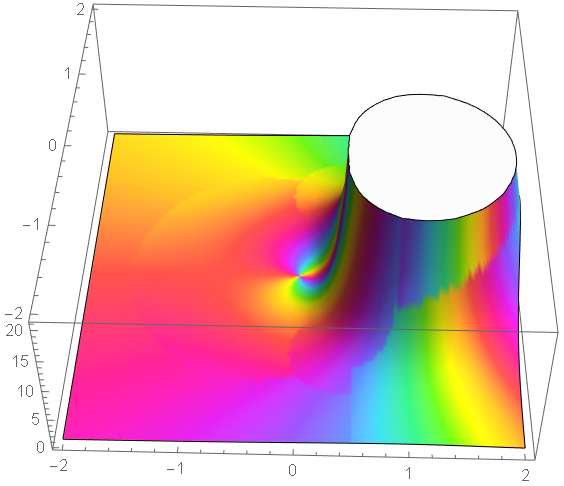
\includegraphics[width=0.75\textwidth]{4.3LHS.png}
 	 	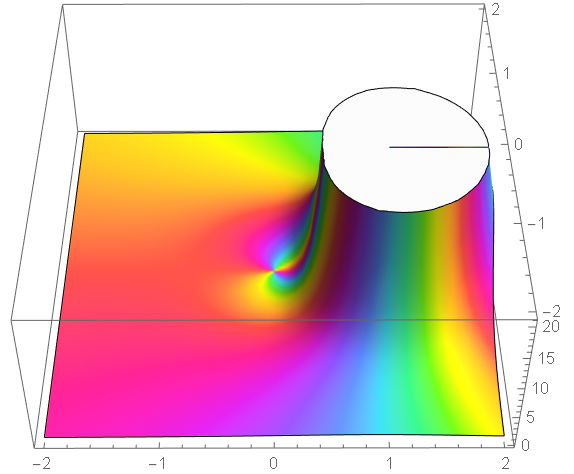
\includegraphics[width=0.75\textwidth]{4.3RHS.png}
 	\caption{The complex plot of the Corollary \ref{4.3.1} for $\mu = \pi + i$, $m=1$ and $n=3$. (Top) The left-hand side of equality. (Bottom) The right-hand side of the equality. For both plots, the $x$-axis refers to the real-part, the $y$-axis define as the imaginary part, the $z$-axis is the absolute value of the expression $\mathrm{Abs}(f)$, and the color refers to the argument of the expression $\mathrm{Arg}(f)$. Both figures generated using Wolfram Mathematica v12.1.}
 	\label{F4.3.1}
 \end{figure}

The above result appears to extend the analyticity outside the region of $|z| < 1$ by the principle of analytic continuation. Again, for accuracy check, we will obtain the complex plot of the left-hand and right-hand side of the equation \eqref{4.3.1e}. From Figure \ref{F4.3.1}, we can see that the complex plot for both sides seems identical too. Both figures is observed to have a zero at $z=0$ and singularity at $z=1$. The only difference we observe is the branch cut along $[1, \infty]$, which is due to the hypergeometric function. Again, the appearance of the branch cut for the complex plot of the right hand side equation is due to the numerical artifacts of the numerical evaluation. 


\subsubsection{Special case: $m = 1$}

If we let $ m = 1$, the Stieltjes transform in equation \eqref{STGHF} will reduce to
\begin{equation}
\int_0^{\infty} \frac{(a+x)^{-\mu}}{(b+x)^{n}} \, \mathrm{d}x = \frac{ \Gamma(\mu+n-1)}{\Gamma(\mu+n)} \frac{b^{1-n}}{a^{\mu}}\, \pFq{2}{1}{\mu,1}{\mu+n}{1-\frac{b}{a}}. 
\label{STGHF}
\end{equation}
Since $m,n$ are positive integers, this special case will always fall under the case of $n \geq m$. Invoking the corollary \ref{4.3.1} and simplifying terms, we will have a reduction formula 
\begin{equation}
	\begin{split} \label{5.64}
    F^{1 \, 1 \, 2}_{1 \, 0 \, 1}&\left[\begin{array}{lll}
	n+\mu &: 1 &; 1,n+\mu-1  \\
	2 &:  &; n+\mu 
	\end{array};\; z,z\right] \\& \hspace{-10mm} - (n+\mu-1) \, F^{1 \, 1 \, 2}_{1 \, 0 \, 1}\left[\begin{array}{lll}
	n+\mu &: 1 &; 1,n  \\
	2&:  &; n+1 
	\end{array};\; z,z\right] \\& \hspace{5mm} =
	 \frac{1}{z} \pFq{1}{0}{n+\mu-1}{}{z} 
	\\& \hspace{20mm} \times \left[ \psi(n) -\psi(n+\mu-1) - \mathrm{Log}(z) \right] 
   \\&\hspace{10mm}- \frac{\Gamma(\mu) (n-1)! (-1)^{1-n}}{\Gamma(n+\mu) \,z^{n}} \pFq{2}{1}{\mu,1}{\mu+n}{1-z}
      \\&\hspace{10mm}+ \frac{\Gamma(\mu)\Gamma(1-\mu)(n-1)!}{\Gamma(n+\mu-1) \, z^{n-\mu} } \\& \hspace{20mm} \times \sum_{k=1}^{n-1}  \frac{(-1)^{1-n}}{k\Gamma(n-k)\Gamma(2-\mu-n+k)} \left( \frac{1-z}{z} \right)^{k-\mu-n+1}.
	\end{split}
	\end{equation}
According to \cite{ancarani2010derivatives}, we can express the Kampé de Fériet function as a differentation of the hypergeometric function with respect to the parameter. Letting $\alpha = n+\mu-1$, the first term of the left hand side can be express as
\begin{equation}
	\begin{split}
    F^{1 \, 1 \, 2}_{1 \, 0 \, 1} \left[\begin{array}{lll}
	\alpha+1 &: 1 &; 1,\alpha  \\
	2 &:  &; \alpha +1
	\end{array};\; z,z\right] & = \frac{\partial }{\partial \alpha} \frac{1}{z} \pFq{1}{0}{\alpha}{}{z}
	\\& = \frac{1}{z} \frac{\partial }{\partial \alpha}  (1-z)^{-\alpha}
	\\& = - \frac{1}{z} \ln{(1-z)} (1-z)^{\alpha}
	\\& = - \frac{1}{z} \ln{(1-z)} \pFq{1}{0}{\alpha}{}{z}.
	\end{split}
	\end{equation}
Substituting the above expression to equation \eqref{5.64}, we will result to
\begin{equation}
	\begin{split} \label{SPP}
     F^{1 \, 1 \, 2}_{1 \, 0 \, 1}&\left[\begin{array}{lll}
	n+\mu &: 1 &; 1,n  \\
	2&:  &; n+1 
	\end{array};\; z,z\right] \\& \hspace{5mm} =
	- \frac{1}{z (n+\mu-1)} \pFq{1}{0}{n+\mu-1}{}{z} 
	\\& \hspace{20mm} \times \left[ \mathrm{Log} \left( \frac{1-z}{z} \right) + \psi(n) -\psi(n+\mu-1) \right] 
   \\&\hspace{10mm}+ \frac{\Gamma(\mu) (n-1)! (-1)^{1-n}}{\Gamma(n+\mu) (n+\mu-1) \,z^{n}} \pFq{2}{1}{\mu,1}{\mu+n}{1-z}
      \\&\hspace{10mm}- \frac{\Gamma(\mu)\Gamma(1-\mu)(n-1)!}{\Gamma(n+\mu) \, z^{n-\mu} } \\& \hspace{20mm} \times \sum_{k=1}^{n-1}  \frac{(-1)^{1-n}}{k\Gamma(n-k)\Gamma(2-\mu-n+k)} \frac{(1-z)^{k-\mu-n+1}}{z^{k+1}} .
	\end{split}
	\end{equation}
The above expression is just the reduction formula of the Kampé de Fériet function found in  \cite{SPP-2020-2G-03}. We create a $3$D plot of the left-hand side and right-hand side of the equation for some accuracy checks. It can be seen in Figure \ref{FSPP} that the plot of both expression have a singularity at $z = 1$ and look the same. The only difference is the two branch cuts on the right hand side plot due to the numerical artifacts of the logarithmic term. The plots confirm the accuracy of the above equation.

\begin{figure}[t]
 	\centering
 	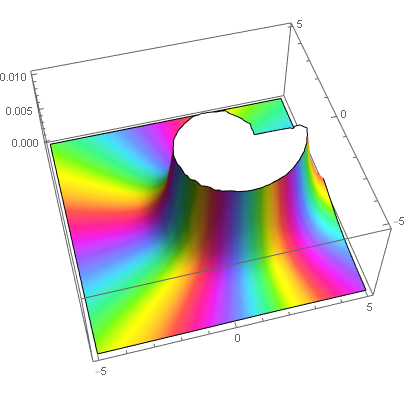
\includegraphics[width=0.6\textwidth]{SPPLHSf.png}
 	 	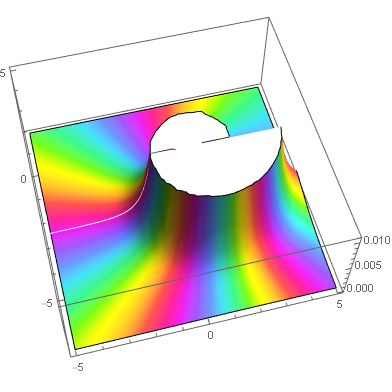
\includegraphics[width=0.6\textwidth]{SPPRHSf.png}
 	\caption{The complex plot of the equation \eqref{SPP} for $\mu = \pi + i$ amd $n=3$. (Top) The left-hand side of equality. (Bottom) The right-hand side of the equality. For both plots, the $x$-axis refers to the real-part, the $y$-axis define as the imaginary part, the $z$-axis is the absolute value of the expression $\mathrm{Abs}(f)$, and the color refers to the argument of the expression $\mathrm{Arg}(f)$. Both figures generated using Wolfram Mathematica v12.1.}
 	\label{FSPP}
 \end{figure}


\subsection{Case 2: $\nu$, $\rho \not \in \mathbb{Z}^{+}$, $\nu-\rho \in \mathbb{Z}$}

We will consider here the case $\mu, \nu, \rho > 0$, and $\nu,\rho \not \in \mathbb{Z}^{+}$. The origin $z=0$ is pole singularity when the difference of $(\nu-\rho)$ is an integer and $z=-b$ is a branch point since $\rho$ is not an integer. We choose the branch cut to run along the positive real axis. Now, we will extract the desired integral from the contour integral 
\begin{equation}
\int_C \frac{z^{\nu-1} (a+z)^{-\mu}}{(b+z)^{\rho}}\,\left(\log z - i\pi\right)\, \mathrm{d}z,
\end{equation}
since the divergence is from a pole singularity. The contour $C$ is shown in Figure \ref{deformation} and will be collapsed into $C'$. The $C'$ contour is evaluated as  
\begin{equation}
\begin{split}
&\int_0^{\infty} \frac{x^{\nu-1} (a+x)^{-\mu}}{(b+x)^{\rho}} \mathrm{d}x=  \frac{1}{2\pi i} \int_C \frac{z^{\nu-1} (a+z)^{-\mu}}{(b+z)^{\rho}}\,\left(\log z - i\pi\right)\, \mathrm{d}z \\
& \hspace{24mm}+ (-1)^{\nu-\rho+1} \frac{\sin(\pi \rho)}{\pi} \lim_{\epsilon\rightarrow 0} \left[\int_0^{b-\epsilon} \frac{x^{\nu-1} (a-x)^{-\mu}}{(b-x)^{\rho}}\,\log(x)\,\mathrm{d}x \right. \\
& \hspace{24mm}\left.  + \frac{e^{-i\pi\nu}}{(1-e^{-2\pi\rho i})}\int_{C_{\epsilon}} \frac{z^{\nu-1} (a+z)^{-\mu}}{(b+z)^{\rho}}\,\left(\log z - i\pi\right)\, \mathrm{d}z\right].
\end{split}
\end{equation}
Again, we recognize that the limit is the finite part of the divergent integral $\int_0^b x^{\nu-1} (a+x)^{-\mu} (b+x)^{-\rho}\,\mathrm{d}x$. Then, the representation reduces to 
\begin{equation}
\begin{split} \label{repcase4b}
&\int_0^{\infty} \frac{x^{\nu-1} (a+x)^{-\mu}}{(b+x)^{\rho}}\mathrm{d}x =  \frac{1}{2\pi i} \int_C \frac{z^{\nu-1} (a+z)^{-\mu}}{(b+z)^{\rho}}\,\left(\log z - i\pi\right)\, \mathrm{d}z \\
& \hspace{24mm}+  (-1)^{\nu-\rho+1}\frac{\sin(\pi\rho)}{\pi} \bbint{0}{b} \frac{x^{\nu-1} \, (a-x)^{-\mu}}{(b-x)^{\rho}} \, \ln(x)\, \mathrm{d}x.
\end{split}
\end{equation}
The equality holds for $a>b>0$, $\mathrm{Re}(\nu) > 0$, $\mathrm{Re}(\rho) > 0$ , $\mu \not = 0$, $(\rho+\mu-\nu)>0$, $\rho \not \in \mathbb{Z}$ and $(\nu-\rho)\in \mathbb{Z}$. Next, we will perform the same expansion in the first term and perform a term by term integration. Similar to the previous case, there are two possible cases, depending on whether all the integrals appearing are finite-part integrals or not. Also, the third term introduces two possible cases depending on the value of $\rho$: If $0<\rho<1$, the integral is just a regular convergent integral; if $\rho\geq 1$, the integral is the finite part of a divergent integral. Nevertheless, we can simultaneously consider the two cases because the finite part coincides with the regular value of the integral when it converges. 

Let us now obtain the finite part integral in equation \eqref{repcase4b}. To determine the convergent and divergent parts of the integral, we let $\epsilon$ be some positive arbitrarily small number and consider the integral
\begin{equation}
\frac{a^{\mu}}{b^{\nu-\rho}}\int_{0}^{b-b\epsilon} \frac{x^{\nu-1} (a-x)^{-\mu}}{(b-x)^{\rho}}\,\ln(x)\, \mathrm{d}x = C_{\epsilon} + D_{\epsilon}.
\end{equation}
In the limit as $\epsilon$ approaches zero, the $C_{\epsilon}$ and $D_{\epsilon}$ are the convergent and divergent parts, respectively. Recall that the assigned finite part is the limit $\lim_{\epsilon\rightarrow 0} C_{\epsilon}$. Performing some change in variable $x=b y$ will reduce the integral into
\begin{equation}\label{integralorig}
\begin{split}
&\frac{a^{\mu}}{b^{\nu-\rho}}\int_0^{b-b\epsilon} \frac{x^{\nu-1} (a-x)^{-\mu}}{(b-x)^{\rho}}\,\ln(x)\, \mathrm{d}x =  \ln(b) \int_0^{1-\epsilon} \frac{y^{\nu-1} (1-\frac{b}{a} y)^{-\mu}}{(1-y)^{\rho}}\, \mathrm{d}y \\
& \hspace{20mm}+\int_0^{1-\epsilon} \frac{y^{\nu-1} \left(1-\frac{b}{a} y\right)^{-\mu}}{(1-y)^{\rho}}\,\ln(y)\,\mathrm{d}y,
\end{split}
\end{equation}
for $b>0$. The above expression will result to a combination of two finite part integrals,
\begin{equation}\label{integralorigx}
\begin{split}
&\frac{a^{\mu}}{b^{\nu-\rho}}\bbint{0}{b} \frac{x^{\nu-1} (a-x)^{-\mu}}{(b-x)^{\rho}}\,\ln(x)\, \mathrm{d}x =  \ln(b) \bbint{0}{1} \frac{y^{\nu-1} (1-\frac{b}{a} y)^{-\mu}}{(1-y)^{\rho}}\, \mathrm{d}y \\
& \hspace{20mm}+\bbint{0}{1} \frac{y^{\nu-1} \left(1-\frac{b}{a} y\right)^{-\mu}}{(1-y)^{\rho}}\,\ln(y)\,\mathrm{d}y .
\end{split}
\end{equation}
The two finite-part integral in the right hand side can be generalized as \begin{equation}
\int_0^{1-\epsilon} \frac{y^{\nu-1} (1-\frac{b}{a} y)^{-\mu}}{(1-y)^{\rho}}\,g_l(y) \mathrm{d}y = C_{\epsilon}^{(l)} + D_{\epsilon}^{(l)}, \;\;\; l=1, 2, 
\end{equation}
where $g_1(y)=1$ and $g_2(y)=\ln(y)$, and the  $C_{\epsilon}^{(l)}$'s and $D_{\epsilon}^{(l)}$'s are the respective converging and diverging parts of the integrals. For the evaluation of this integrals, we let $b/a<(1-\epsilon)$ and expand $(1-b y/a)^{-\mu}$ at the origin. Then, we will interchange the order of integral and summation to perform a term by term integration. The interchanging of the operators is allowed since the series is uniformly convergent along the interval of integration $[0,1-\epsilon]$,
\begin{align}
\begin{split}
    \int_0^{1-\epsilon} & \frac{y^{\nu-1} (1-\frac{b}{a} y)^{-\mu}}{(1-y)^{\rho}} \,g_l(y)\,  \mathrm{d}y \\& = \sum_{k=0}^{\infty} (-1)^k {-\mu \choose k}\left(\frac{b}{a}\right)^k \int_0^{1-\epsilon} \frac{y^{\nu-1+k}}{(1-y)^{\rho}}\,g_l(y)\,\mathrm{d}y.    
\end{split}
\end{align}
This lead us to evaluate the integrals
\begin{equation}\label{rawintegral}
\int_0^{1-\epsilon} \frac{y^{\nu+k-1}}{(1-y)^{\rho}}\,g_l(y)\,\mathrm{d}y=\tilde{C}^{(l)}_{k,\epsilon} + \tilde{D}^{(l)}_{k,\epsilon},
\end{equation}
where the $\tilde{C}^{(l)}_{\epsilon}$'s and $\tilde{D}^{(l)}_{\epsilon}$'s are the converging and diverging parts of the integrals for a given $k$. The converging parts of $C_{\epsilon}$ will obviously come from the converging parts of $\tilde{C}_{k,\epsilon}$'s. Therefore, when the infinite series converges, the finite integrals are given by
\begin{equation}\label{fpixxx}
\bbint{0}{1}\frac{y^{\nu-1} (1-\frac{b}{a} y)^{-\mu}}{(1-y)^{\rho}}\, \mathrm{d}y = \sum_{k=0}^{\infty} (-1)^k {-\mu \choose k}\left(\frac{b}{a}\right)^k \bbint{0}{1} \frac{y^{\nu-1+k}}{(1-y)^{\rho}}\,\mathrm{d}y ,
\end{equation}
\begin{equation}\label{fpixxx2}
\bbint{0}{1}\frac{y^{\nu-1} (1-\frac{b}{a} y)^{-\mu}}{(1-y)^{\rho}}\,\ln(y)\, \mathrm{d}y = \sum_{k=0}^{\infty} (-1)^k {-\mu \choose k}\left(\frac{b}{a}\right)^k \bbint{0}{1} \frac{y^{\nu-1+k}}{(1-y)^{\rho}}\,\ln(y)\,\mathrm{d}y.
\end{equation}
The task now is evaluate this two finite-part integrals
\begin{equation}
\bbint{0}{1} \frac{y^{\nu-1+k}}{(1-y)^{\rho}}\,\mathrm{d}y,\;\;\;
%\end{equation}
%\begin{equation}
\bbint{0}{1} \frac{y^{\nu-1+k}}{(1-y)^{\rho}}\,\ln(y)\,\mathrm{d}y.
\end{equation}
Observe that the only difference between the two finite-part integrals is the logarithmic factor and this factor can be generated through differentiation. Hence, the second finite-part integrals can be obtained from the differentiation of the first finite-part integral. 

To evaluate the first finite-part integral, we will consider the finite-part integral 
\begin{equation}
\bbint{0}{1}\frac{y^{\sigma-1}}{(1-y)^{\rho}}\,\mathrm{d}y.
\end{equation}
where $\mathrm{Re}(\sigma)>0$ and $\mathrm{Re}(\rho)>0$. Then, we consider the usual integral 
\begin{equation} \label{fp1}
\int_0^{1-\epsilon} \frac{y^{\sigma-1}}{(1-y)^{\rho}}\,\mathrm{d}y
\end{equation} 
where $0<\epsilon<1$. To completely evaluate the above integral, we will use the two facts about beta function $B(a,b)$, its integral representation
\begin{equation}\label{betaintegrep}
B_{z}(a,b) = \int_0^z t^{a-1} (1-t)^{b-1}\,\mathrm{d}t,\; \mathrm{Re}(a)>0,
\end{equation}
and its behavior in the neighbhood of $z=1$.
\begin{equation}\label{betainc1}
B_z(a,b)= B(a,b) - \frac{(1-z)^{b} z^a}{b}\left(1+O(z-1)\right),
\end{equation}
Comparing the integral \eqref{fp1} from the integral representation of Beta function in \eqref{betaintegrep}, we will obtain the integral \eqref{fp1} as the incomplete beta function with $z=1-\epsilon$, $a=\sigma$ and $b=1-\rho$
\begin{equation} \label{fp12}
    \int_{0}^{1-\epsilon} \frac{y^{\sigma-1}}{(1-y)^{\rho}} \,\mathrm{d}y = B_{1-\epsilon}(\sigma, 1-\rho).
\end{equation}
Then, invoking the expansion of the beta funtion \eqref{betainc1} at $z=1$, the integral \eqref{fp12} will results to
\begin{align}
    \int_0^{1-\epsilon} \frac{y^{\sigma-1}}{(1-y)^{\rho}}\,\mathrm{d}y & = B(\sigma, 1-\rho) - \frac{\epsilon^{1-\rho} (1-\epsilon)^{\sigma}}{1-\rho} + \left(1+O(-\epsilon)\right)
    \\& =\frac{\pi\Gamma(\sigma)}{\sin(\pi\rho) \Gamma(\rho) \Gamma(1+\sigma-\rho)} + O(\epsilon^{1-\rho}),
\end{align}
where we made a further simplification using the fact that $\rho$ is a non-integer. If $\mathrm{Re}(\rho)<1$, the second term will just approach to zero as $\epsilon \to 0$. It implies that the finite-part integral is a converging integral, and it will just take its value. While, when $\mathrm{Re}(\rho)>1$, the second term will diverge. In this case, the finite-part integral will be obtained by dropping the diverging part and performing the limit $\epsilon \to 0$ to the converging part. Thus we arrive at the finite part integral
\begin{equation}\label{fpingteg1x}
\bbint{0}{1}\frac{y^{\sigma-1}}{(1-y)^{\rho}}\,\mathrm{d}y = \frac{\pi\Gamma(\sigma)}{\sin(\pi\rho) \Gamma(\rho) \Gamma(1+\sigma-\rho)},
\end{equation}
for $\mathrm{Re}(\sigma)>0$ and $\mathrm{Re}(\rho)>0$. Since $1/\Gamma(z)=0$ for $z \in \mathbb{Z}_{0}^{-}$, the finite part assumes the zero value for $1+\sigma-\rho\in \mathbb{Z}_{0}^{-}$. Explicitly, we have
\begin{equation}\label{fpingteg1xxx}
\bbint{0}{1}\frac{y^{\sigma-1}}{(1-y)^{\rho}}\,\mathrm{d}y = 0,
\end{equation}
for $\sigma - \rho \in \mathbb{Z}_{0}^{-}$.

For the calculation of the second finite-part integral, we will perform some classic Feymann tricks. Inspecting the integral, we can see that that the integral the two integral is related by some differentiation of the parameter. Using the fact that 
\begin{equation}
    \frac{\partial}{\partial \nu} y ^{\nu-1} =  y^{\nu-1}\, \ln{y} \
\end{equation}
we can establish the following relation
\begin{equation}
    \frac{\partial}{\partial\nu} \, \int_0^{1-\epsilon}  \frac{y^{\nu-1}} {(1-y)^{\rho}}\,\mathrm{d}y =  \int_0^{1-\epsilon}  \frac{y^{\nu-1}} {(1-y)^{\rho}} \ln y \,\mathrm{d}y. 
\end{equation}
This relation confirms by the converges of the integral along the entire integration interval $[0,1-\epsilon]$. Therefore, the second finite part in the right hand side of equation \eqref{integralorigx} is just the differentiation with respect to $\nu$ of the finite-part integral \eqref{fpingteg1x}. Performing the differentiation on equation \eqref{fpingteg1x}, we obtain the second finite-part integral as
\begin{equation}\label{fpingteg1xxx2}
\bbint{0}{1}\frac{y^{\sigma-1}}{(1-y)^{\rho}}\,\ln(y)\,\mathrm{d}y = \frac{\pi\Gamma(\sigma)}{\sin(\pi\rho) \Gamma(\rho) \Gamma(1+\sigma-\rho)} \left(\psi(\sigma)-\psi(\sigma-\rho+1)\right),
\end{equation}
for $\mathrm{Re}(\sigma)>0$ and $\mathrm{Re}(\rho)>0$ and non-integer $\rho$. For $\sigma-\rho+1 \in \mathbb{Z}_{0}^{-}$, we will have a removable singularity  
\begin{equation}
    \lim_{z\rightarrow -n} \frac{\psi(z)}{\Gamma(z)} = (-1)^{n+1} n!,
\end{equation}
for a positive integer $n$. This yields the finite part integral
\begin{equation}\label{fpingteg1xx3}
\bbint{0}{1}\frac{y^{\sigma-1}}{(1-y)^{\rho}}\,\ln(y)\,\mathrm{d}y = (-1)^{\rho-\sigma+1} \frac{\pi\Gamma(\sigma) (\rho-\sigma-1)!}{\sin(\pi\rho) \Gamma(\rho)},
\end{equation}
for $(\sigma-\rho) \in \mathbb{Z}_{0}^{-}$.

Inspecting all the finite-part integral, it is observed that all finite-part integral depends on the difference of the parameters $\rho$ and $\nu$. Thus,  we will consider separately the cases $(\nu-\rho) \in \mathbb{Z}^{+}$ and $(\rho-\nu) \in \mathbb{Z}_{0}^{-}$.  

\subsubsection{Case $(\nu-\rho) \in \mathbb{Z}^{+}$}

For this case, the expansion in the equation \eqref{repcase4b} decomposes into a finite series of convergent integrals and an infinite series of finite part integrals. The expansion assumes the form
\begin{equation}
\begin{split} 
\int_0^{\infty} \frac{x^{\nu-1} (a+x)^{-\mu}}{(b+x)^{\rho}} \mathrm{d}x  = &  \sum_{k=0}^{(\nu-\rho)-1} \, {- \rho \choose k} \, b^{k} \int_0^{\infty} \ \frac{(a+x)^{-\mu}}{x^{k+\rho-\nu+1}} \,\mathrm{d}x \\& + \sum_{k=(\nu-\rho)}^{\infty} {- \rho \choose k} \, b^{k} \, \bbint{0}{\infty} \frac{(a+x)^{-\mu}}{x^{k+\rho-\nu+1}} \,\mathrm{d}x
\\&- (-1)^{\nu-\rho}\frac{\sin(\pi\rho)}{\pi} \bbint{0}{b} \frac{x^{\nu-1} \, (a-x)^{-\mu}}{(b-x)^{\rho}} \, \ln(x)\, \mathrm{d}x.
\label{case4b}
\end{split}
\end{equation}
From the definition of beta function, the integrals in the first group of terms evaluate to
\begin{equation}
    \int_0^{\infty} \frac{(a+x)^{-\mu}}{x^{k+\rho-\nu+1}}\,\mathrm{d}x = \frac{\Gamma(\nu-\rho-k)\Gamma(k+\mu-\nu+\rho)}{a^{k+\mu+\nu-\rho} \Gamma(\mu)},
\end{equation}
for $k=0, \dots, (\nu-\rho-1)$. On the other hand, the finite part integrals in the second term is given by the equation \eqref{fp} with the substitution $n-m \to \rho-\nu$. This will give us
\begin{equation}
\begin{split} \label{second}
    \bbint{0}{\infty} \frac{(a+x)^{-\mu}}{x^{k+\rho-\nu+1}} \,\mathrm{d}x &= \frac{1}{a^{k+\rho-\nu+\mu}} {-\mu \choose k+\rho-\nu} \\
    &\times\left[\ln(a) + \psi(k+\rho-\nu+1)-\psi(k+\rho-\nu+\mu)\right]
    \end{split}
\end{equation}
for $=(\nu-\rho), (\nu-\rho+1),\dots$. We can now further simplify this two group terms of equation \eqref{case4b}. Substituting the values of the convergent integrals, the first term will become
\begin{equation}\label{xxx1}
\begin{split}
    &\sum_{k=0}^{(\nu-\rho)-1} \, {- \rho \choose k} \, b^{k} \int_0^{\infty} \ \frac{(a+x)^{-\mu}}{x^{k+\rho-\nu+1}} \,\mathrm{d}x \\
    &\hspace{8mm}= \frac{1}{a^{\mu-\nu+\rho} \Gamma(\mu)} \sum_{k=0}^{\nu-\rho-1} {-\rho \choose k} \Gamma(\nu-\rho-k) \Gamma(k+\mu-\nu+\rho) \left(\frac{b}{a}\right)^k
    \end{split}
\end{equation}
Writing the binomial coefficient in terms of the gamma function and using the identity $\Gamma(z-n) = (-1)^{n} \Gamma(z)/(1-z)_n$, the right hand side of equation simplifies to
\begin{equation}\label{xxx1v2}
\begin{split}
    &\sum_{k=0}^{(\nu-\rho)-1} \, {- \rho \choose k} \, b^{k} \int_0^{\infty} \ \frac{(a+x)^{-\mu}}{x^{k+\rho-\nu+1}} \,\mathrm{d}x \\
    &\hspace{8mm}= \frac{\Gamma(\nu-\rho) \Gamma(\mu-\nu+\rho)}{a^{\mu+\rho-\nu}\Gamma(\mu)} \sum_{k=0}^{\nu-\rho-1} \frac{(\rho)_k (\mu-\nu+\rho)_k}{(1-\nu+\rho)_k k!} \left(\frac{b}{a}\right)^k.
       \end{split}
\end{equation}
For the second group of terms, we substitute the evaluated finite part integrals in equation \eqref{second}. Next is to shift the index of summation from $k$ to $k+\nu-\rho$ so that we can easily transform it into a hypergeometric function. Then, we write all binomial coefficients in terms of the gamma function. This will result to
\begin{equation}
    \begin{split} \label{xxx2}
        &\sum_{k=(\nu-\rho)}^{\infty} {- \rho \choose k} \, b^{k} \, \bbint{0}{\infty} \frac{(a+x)^{-\mu}}{x^{k+\rho-\nu+1}} \,\mathrm{d}x\\
        &\hspace{4mm}= 
    \frac{b^{\nu-\rho}}{a^{\mu}} \frac{(-1)^{\nu-\rho}}{\Gamma(\mu) \Gamma(\rho)} \sum_{k=0}^{\infty} \frac{\Gamma(k+\mu) \Gamma(k+\nu)}{\Gamma(k+\nu-\rho+1) k!} \\& \hspace{10mm} \times \left[\ln{a}+\psi(k+1)-\psi(k+\mu)\right]\left(\frac{b}{a}\right)^k.
    \end{split}
\end{equation}
The infinite series converges for all $|b/a|<1$ and $\mathrm{Re}(\rho-\nu+\mu)>0$.

Finally, we evaluate the last term of equation \eqref{case4b}. Under the condition that $(\nu-\rho)$ is a positive integer, and with $\sigma=\nu+k$, the finite-part integral \eqref{fpingteg1x} does not vanish for all $k=0, 1, \dots$. Substituting the finite parts \eqref{fpingteg1x} back into equation \eqref{fpixxx} yields 
\begin{equation}\label{integralseries}
    \bbint{0}{1} \frac{y^{\nu-1} (1-\frac{b}{a} y)^{-\mu}}{(1-y)^{\rho}}\, \mathrm{d}y =\frac{\pi}{\sin(\pi\rho)\Gamma(\mu)\Gamma(\rho)}\sum_{k=0}^{\infty} \frac{\Gamma(k+\mu) \Gamma(k+\nu)}{\Gamma(1+k+\nu-\rho) k!} \left(\frac{b}{a}\right)^k ,
\end{equation}
for $b/a<1$, where the binomial coefficient has been written in terms of the gamma function to arrive at this expression. To extend the result to accommodate the case $b/a>1$, we perform a hypergeometric summation to the infinite series to give  
\begin{equation}\label{integralclosed}
    \bbint{0,}{1} \frac{y^{\nu-1} (1-\frac{b}{a} y)^{-\mu}}{(1-y)^{\rho}}\, \mathrm{d}y= \frac{\pi \Gamma(\nu)}{\sin(\pi \rho) \Gamma(\rho) \Gamma(1+\nu-\rho)} \, \pFq{2}{1}{\mu,\nu}{1+\nu-\rho}{\frac{b}{a}} ,
\end{equation}

Similarly the finite part integral is given by equation \eqref{fpingteg1xx3} for all $k$. Then substituting the finite part into equation, the logarithmic finite part integral is given by
\begin{equation}\label{integrallogseries}
\begin{split}
    &\bbint{0}{1} \frac{y^{\nu-1} (1-\frac{b}{a} y)^{-\mu}}{(1-y)^{\rho}}\,\ln(y)\, \mathrm{d}y=\frac{\pi}{\sin(\pi\rho) \Gamma(\mu)\Gamma(\rho)} \\ 
    &\hspace{18mm}\times\sum_{k=0}^{\infty} \frac{\Gamma(k+\mu) \Gamma(k+\nu)}{\Gamma(1+k+\nu-\rho) k!}  \left[\psi(k+\nu)-\psi(1+k+\nu-\rho)\right] \left(\frac{b}{a}\right)^k ,
    \end{split}
\end{equation}
for $\rho>1$ or the regular value when $\rho<1$; this result is valid for $b/a<1$. The extension of this result for $b/a>1$ can be obtained by differentiating equation \eqref{integralclosed} with respect to $\nu$.

Again, the two finite-part integral above are the finite-part of the singular contribution. Substituting those finite part to the equation \eqref{integralorigx} will result to
\begin{equation}
\begin{split}
&\frac{a^{\mu}}{b^{\nu-\rho}} \bbint{0}{b} \frac{x^{\nu-1} \, (a-x)^{-\mu}}{(b-x)^{\rho}} \, \ln(x)\, \mathrm{d}x\\
&\hspace{20mm}= \frac{\pi \Gamma(\nu)}{\sin(\pi \rho) \Gamma(\rho) \Gamma(1+\nu-\rho)} \, \pFq{2}{1}{\mu,\nu}{1+\nu-\rho}{\frac{b}{a}}\ln(b) \\
&\hspace{24mm}+ \frac{\pi}{\sin(\pi\rho) \Gamma(\mu)\Gamma(\rho)}  
\sum_{k=0}^{\infty} \frac{\Gamma(k+\mu) \Gamma(k+\nu)}{\Gamma(1+k+\nu-\rho) k!}\\  
&\hspace{30mm}\times \left[\psi(k+\nu)-\psi(1+k+\nu-\rho)\right] \left(\frac{b}{a}\right)^k.
\end{split}
\end{equation} 
We substitute this back into expression \eqref{case4b}, together with equations \eqref{xxx1} and \eqref{xxx2}. The coefficient of $\ln{a}$ can be rewritten as a hypergeometric function and combined to $\ln{b}$. Then, we will replace 
$b/a$ with complex number $z$ and invoke the principle of analytic continuation. Similar to the other parameters $\mu$, $\nu$ and $\rho$, the parameters can be a complex number, provided that $\nu$ and $\rho$ are non-integer and $(\nu-\rho)\in\mathbb{Z}^+$. Doing so, we will obtain the equation
\begin{equation}
    \begin{split}
        & \frac{\Gamma(\nu)\Gamma(\mu-\nu+\rho)}{\Gamma(\mu+\rho)} \pFq{2}{1}{\mu,\nu}{\mu+\rho}{1-z} \\&\hspace{10mm}= \frac{\Gamma(\nu-\rho)\Gamma(\mu-\nu+\rho)}{\Gamma(\mu) z^{\nu-\rho}} \sum_{k=0}^{\nu-\rho-1} \frac{(\rho)_k (\mu-\nu+\rho)_k}{(1-\nu+\rho)_k k!} z^k \\
        &\hspace{10mm}-(-1)^{\nu-\rho} \frac{\Gamma(\nu)}{\Gamma(\rho) \Gamma(\nu-\rho+1)}  \,\mathrm{Log}(z) \sum_{k=0}^{\infty} \frac{(\mu)_k (\nu)_k}{(\nu-\rho+1)_k k!} z^k \\
        &\hspace{10mm}+ (-1)^{\nu-\rho}\frac{\Gamma(\nu)}{\Gamma(\rho) \Gamma(\nu-\rho+1)}  \sum_{k=0}^{\infty} \frac{(\mu)_k (\nu)_k}{(\nu-\rho+1)_k k!}\\
        &\hspace{15mm}\times\left[\psi(k+1)-\psi(k+\mu)+\psi(k+\nu+1-\rho)-\psi(k+\nu)\right] z^k .
    \end{split}
\end{equation}
Again, we can further simplify it by using the definition of $_{p}\tilde{\psi}_{q}$ in equation \eqref{psi} and expressing the other series in terms of hypergeometric function. Therefore, we will have a theorem.


\begin{theorem} \label{4.4}
Let $\mu$ be any positive number, $\nu$ and $\rho$ be positive non-integer, with $(\nu-\rho)=1, 2, \dots$ and $(\mu-\nu+\rho)\neq 0, -1, -2, \dots$. Then
\begin{equation}
    \begin{split}
        & \frac{\Gamma(\nu)\Gamma(\mu-\nu+\rho)}{\Gamma(\mu+\rho)} \pFq{2}{1}{\mu,\nu}{\mu+\rho}{1-z} \\&\hspace{10mm}= \frac{\Gamma(\nu-\rho)\Gamma(\mu-\nu+\rho)}{\Gamma(\mu) z^{\nu-\rho}} \sum_{k=0}^{\nu-\rho-1} \frac{(\rho)_k (\mu-\nu+\rho)_k}{(1-\nu+\rho)_k k!} z^k \\
        &\hspace{10mm}-(-1)^{\nu-\rho} \frac{\Gamma(\nu)}{\Gamma(\rho) \Gamma(\nu-\rho+1)}  \,\mathrm{Log}(z) \pFq{2}{1}{\mu, \nu}{\nu-\rho-1}{z} \\
        &\hspace{10mm}+ (-1)^{\nu-\rho}\frac{\Gamma(\nu)}{\Gamma(\rho) \Gamma(\nu-\rho+1)}  \Bigg[ \pPq{2}{1}{\mu,\nu}{\nu-\rho-1}{1}{z}\\
        &\hspace{30mm} + \pPq{2}{1}{\mu,\nu}{\nu-\rho-1}{\nu-\rho-1}{z}
        \\&\hspace{30mm} - \pPq{2}{1}{\mu,\nu}{\nu}{\mu}{z}- \pPq{2}{1}{\mu,\nu}{\nu-\rho-1}{\mu}{z} \Bigg].
    \end{split}
\end{equation}
for all $z$ such that $z\not =1$. All the functions involve are taken as their principal value. 
\end{theorem}
\noindent The above theorem was already presented in \cite{doi:10.1063/5.0038274} and it is a known Gauss hypergeometric transformation. To obtain a reduction formulas of the Kampé de Fériet Function, we will use again the relation in equation \eqref{DxK}. The following relation can be generated:

\begin{align}
\begin{split}
    &\pPq{2}{1}{\mu,\nu}{\nu-\rho-1}{1}{z} \\&\hspace{10mm} =  -\gamma \, \pFq{2}{1}{\mu,\nu}{\nu-\rho+1}{z}    + z\, \frac{\mu \, \nu}{\nu-\rho+1} \\& \hspace{15mm} \times  F^{2 \, 1 \, 2}_{2 \, 0 \, 1}\left[\begin{array}{lll}
	\mu+1, \nu+1 &: 1 &; 1,1  \\
	2, \nu-\rho+2&:  &; 2 
	\end{array};\; z,z\right],
\end{split}
\end{align}
\begin{align}
\begin{split}
    &\pPq{2}{1}{\mu,\nu}{\nu-\rho-1}{\mu}{z} \\&\hspace{10mm} =  \psi(\mu) \, \pFq{2}{1}{\mu,\nu}{\nu-\rho+1}{z}    + z\, \frac{\nu}{\nu-\rho+1} \\& \hspace{15mm} \times  F^{2 \, 1 \, 2}_{2 \, 0 \, 1}\left[\begin{array}{lll}
	\mu+1, \nu+1 &: 1 &; 1,\mu  \\
	2, \nu-\rho+2&:  &; \mu+1 
	\end{array};\; z,z\right],
\end{split}
\end{align}
\begin{align}
\begin{split}
    &\pPq{2}{1}{\mu,\nu}{\nu-\rho-1}{\nu}{z} \\&\hspace{10mm} =  \psi(\nu) \, \pFq{2}{1}{\mu,\nu}{\nu-\rho+1}{z}    + z\, \frac{\mu}{\nu-\rho+1} \\& \hspace{15mm} \times  F^{2 \, 1 \, 2}_{2 \, 0 \, 1}\left[\begin{array}{lll}
	\mu+1, \nu+1 &: 1 &; 1,\nu  \\
	2, \nu-\rho+2&:  &; \nu+1 
	\end{array};\; z,z\right],
\end{split}
\end{align}
and
\begin{align}
\begin{split}
    & \pPq{2}{1}{\mu,\nu}{\nu-\rho-1}{\nu-\rho-1}{z} \\& \hspace{10mm} =  \psi(\nu-\rho+1) \, \pFq{2}{1}{\mu,\nu}{\nu-\rho+1}{z}    + z\, \frac{\mu \, \nu}{(\nu-\rho+1)^{2}} \\& \hspace{15mm} \times  F^{2 \, 1 \, 2}_{2 \, 0 \, 1}\left[\begin{array}{lll}
	\mu+1, \nu+1 &: 1 &; 1,\nu-\rho+1  \\
	2, \nu-\rho+2&:  &; \nu-\rho+2 
	\end{array};\; z,z\right],
\end{split}
\end{align}

Using the above relation and expressing the infinite series as a hypergeometric function, we will obtain a corollary of theorem \ref{4.4}. 

\begin{corollary} \label{4.4.1}
Let $\nu$ and $\rho$ be positive non-integers with $\nu>\rho$, and $\mu$ a complex number with $(\mu-\nu+\rho)\neq 0, -1, -2, \dots$. Then
	\begin{equation}
	\begin{split}
     F^{2 \, 1 \, 2}_{2 \, 0 \, 1} & \left[\begin{array}{lll}
	\mu+1, \nu+1 &: 1 &; 1,\nu-\rho+1 \\
	2, \nu-\rho+2&:  &; \nu-\rho+2 
	\end{array};\; z,z\right] \\& \hspace{-10mm} - \frac{\nu-\rho+1}{\mu} \,  F^{2 \, 1 \, 2}_{2 \, 0 \, 1}\left[\begin{array}{lll}
	\mu+1, \nu+1 &: 1 &; 1,\nu  \\
	2, \nu-\rho+2&:  &; \nu+1
	\end{array};\; z,z\right]
	\\& \hspace{-10mm} - \frac{\nu-\rho+1}{\nu} \,  F^{2 \, 1 \, 2}_{2 \, 0 \, 1}\left[\begin{array}{lll}
	\mu+1, \nu+1 &: 1 &; 1,\mu  \\
	2, \nu-\rho+2&:  &; \mu+1 
	\end{array};\; z,z\right]
	\\& \hspace{-10mm} + \nu-\rho+1 \,  F^{2 \, 1 \, 2}_{2 \, 0 \, 1}\left[\begin{array}{lll}
	\mu+1, \nu+1 &: 1 &; 1,1  \\
	2, \nu-\rho+2&:  &; 2
	\end{array};\; z,z\right]
	\\& \hspace{5mm} =
	\frac{(\nu-\rho+1) \Gamma(\nu-\rho+2) \Gamma(\rho) \Gamma(\mu-\nu+\rho) \Gamma(\nu-\rho) }{\Gamma(\mu+1) \Gamma(\nu+1) (-z)^{\nu-\rho+1}} \\&\hspace{15mm} \times \sum_{k=0}^{\nu-\rho+1} \frac{(\rho)_{k}(\mu-\nu+\rho)_{k}}{(1-\nu+\rho)_k k!} z^{k}
	\\&\hspace{10mm}+ (-1)^{\nu+\rho}  \frac{1-\rho+\nu}{\mu \, \nu \, z} \frac{\Gamma(\rho)\Gamma(\nu-\rho+1)\Gamma(\mu-\nu+\rho)}{\Gamma(\mu+\rho)}  \\& \hspace{15mm} \times \pFq{2}{1}{\nu,\mu}{\mu+\rho}{1-z}
     \\&\hspace{10mm}- \frac{(1-\rho+\nu)^{2}}{\mu \, \nu \, z} \pFq{2}{1}{\mu, \nu}{\nu-\rho+1}{z}
	\\& \hspace{15mm} \times \left[ \mathrm{Log}(z) + \psi(\rho-\nu+1)-\psi(\rho-\nu+\mu)-\psi(\rho)-\gamma \right].
	\end{split}
	\end{equation}
	for all $z \not = 1$ and $|\mathrm{arg}(z)|<\pi$. All the functions involve are taken as their principal value.  
\end{corollary}

The analyticity of the above function looks to extend outside the region of $|z| < 1$ by the virtue of analytic continuation. This extension was confirmed numerically through Wolfram Mathematica $12.1$.. Additionally, the theorem in this case was numerically confirmed using the same computing software.

\subsubsection{Case $(\rho-\nu) \in \mathbb{Z}^{+}_{0}$ }

Under this condition, the expansion will purely have a finite-part integrals. We will have the expansion
\begin{equation}
\begin{split}
 &\int_0^{\infty} \frac{x^{\nu-1} (a+x)^{-\mu}}{(b+x)^{\rho}} \mathrm{d}x =  \sum_{k=0}^{\infty} {- \rho \choose k} \, b^{k} \, \bbint{0}{\infty} \frac{(a+x)^{-\mu}}{x^{k+\rho-\nu+1}} \,\mathrm{d}x
\\
& \hspace{24mm}- (-1)^{\nu-\rho}\frac{\sin(\pi\rho)}{\pi} \bbint{0}{b} \frac{x^{\nu-1} \, (a-x)^{-\mu}}{(b-x)^{\rho}} \, \ln(x)\, \mathrm{d}x.
\label{case4c}
\end{split}
\end{equation}
Again, the finite-part integral is already evaluated in equation \eqref{fp}. Substituting it to the infinite series we will have
\begin{equation}
\begin{split}
&\sum_{k=0}^{\infty} {- \rho \choose k} \, b^{k} \, \bbint{0}{\infty} \frac{(a+x)^{-\mu}}{x^{k+\rho-\nu+1}} \,\mathrm{d}x \\
&\hspace{12mm} = \frac{(-1)^{\rho-\nu}}{a^{\rho-\nu+\mu}} \frac{\Gamma(\mu+\rho-\nu)}{\Gamma(\mu) \Gamma(\rho-\nu+1)} \sum_{k=0}^{\infty} \frac{(\rho)_k (\mu+\rho-\nu)_k}{(\rho-\nu+1)_k k!} \\
&\hspace{18mm}\times\left[\ln{a} +\psi(k+\rho-\nu+1)-\psi(k+\rho-\nu+\mu)\right] \left(\frac{b}{a}\right)^k .
\label{case4cx}
\end{split}
\end{equation}
The singular contribution will be evaluated similar to the previous case. The first finite-part is given by equation \eqref{fpingteg1x}. This finite-part will have a zero value from $k=0$ to $k = \rho-\nu-1$ because of the factor $\frac{1}{\Gamma(1+k=\nu-\rho)}$. Therefore, the non-zero value will start at $k = \rho-\nu$ that will result to
\begin{equation}
\bbint{0}{1} \frac{y^{\nu-1} (1-\frac{b}{a}y)^{-\mu}}{(1-y)^{\rho}}\,\mathrm{d}y = \frac{\pi \Gamma(\rho-\nu+\mu)}{\sin(\pi \rho) \Gamma(\mu)} \sum_{k=0}^{\infty} \frac{(\mu)_k(\rho)_k}{(k+\rho-\nu)!k!} \left(\frac{b}{a}\right)^{k+\rho-\nu} ,
\end{equation}
Next, the finite-part integral with a logarithmic factor. The value of this finite-part integral will also based on the value of $k$. Using the results in equation \eqref{fpingteg1xx3}, the finite-part integral can be evaluated as 
\begin{equation}
\begin{split}
&\bbint{0}{1} \frac{y^{\nu-1} (1-\frac{b}{a}y)^{-\mu}}{(1-y)^{\rho}}\,\ln(y)\,\mathrm{d}y\\ &\hspace{14mm}=(-1)^{\rho-\nu} \frac{\pi \Gamma(\nu)}{\sin(\pi\rho) \Gamma(\rho)} \sum_{k=0}^{\rho-\nu-1} \frac{(\mu)_k (\nu)_k (\rho-\nu-k-1)!}{k!}\left(-\frac{b}{a}\right)^k\\
&\hspace{18mm} +\frac{\pi \Gamma(\rho-\nu+\mu)}{\sin(\pi\rho) \Gamma(\mu) \Gamma(\rho-\nu+1)} \left(\frac{b}{a}\right)^{\rho-\nu} \sum_{k=0}^{\infty} \frac{(\rho-\nu+\mu)_k (\rho)_k}{(\rho-\nu+1)_k k!} \\
&\hspace{34mm}\times \left[\psi(k+\rho)-\psi(k+1)\right]\left(\frac{b}{a}\right)^k
\end{split}
\end{equation}
for $b/a < 1$.
Combining the two results above will yields to the singular contribution 
\begin{equation}
\begin{split}
&\frac{a^{\mu}}{b^{\nu-\rho}} \bbint{0}{b} \frac{x^{\nu-1} \, (a-x)^{-\mu}}{(b-x)^{\rho}} \, \ln(x)\, \mathrm{d}x\\
&\hspace{10mm}=\frac{\pi \Gamma(\rho-\nu+\mu)}{\sin(\pi\rho) \Gamma(\mu) \Gamma(\rho-\nu+1)}  \sum_{k=0}^{\infty} \frac{(\rho-\nu+\mu)_k (\rho)_k}{(\rho-\nu+1)_k k!}\left(\frac{b}{a}\right)^{k+\rho-\nu}\,\ln(b)\\
&\hspace{12mm}+(-1)^{\rho-\nu} \frac{\pi \Gamma(\nu)}{\sin(\pi\rho) \Gamma(\rho)} \sum_{k=0}^{\rho-\nu-1} \frac{(\mu)_k (\nu)_k (\rho-\nu-k-1)!}{k!}\left(-\frac{b}{a}\right)^k\\
&\hspace{12mm} +\frac{\pi \Gamma(\rho-\nu+\mu)}{\sin(\pi\rho) \Gamma(\mu) \Gamma(\rho-\nu+1)} \left(\frac{b}{a}\right)^{\rho-\nu} \sum_{k=0}^{\infty} \frac{(\rho-\nu+\mu)_k (\rho)_k}{(\rho-\nu+1)_k k!} \\
&\hspace{34mm}\times \left[\psi(k+\rho)-\psi(k+1)\right]\left(\frac{b}{a}\right)^k
\end{split}
\end{equation} 
Collecting all the evaluated finite-part integral and combining the logarithmic term, we will find that all terms are expressed in $b/a$. We will let $z = b/a$ and use the principle of analytic continuation to extend the domain into the complex plane. Also, the parameters will also extended to the complex plane by using the same principle. 
\begin{equation}\label{resultxv0}
\begin{split}
&\frac{\Gamma(\nu)\Gamma(\mu+\rho-\nu)}{\Gamma(\mu+\rho)} \pFq{2}{1}{\mu,\nu}{\mu+\rho}{1-z}\\
&\hspace{8mm} = \frac{\Gamma(\nu)}{\Gamma(\rho)} \sum_{k=0}^{\rho-\nu-1} (-1)^k \frac{(\mu)_k (\nu)_k(\rho-\nu-k-1)!}{k! } z^k  \\
&\hspace{12mm}- \frac{\Gamma(\rho-\nu+\mu)}{\Gamma(\mu)\Gamma(\rho-\nu+1)} (-z)^{\rho-\nu} \sum_{k=0}^{\infty} \frac{(\rho)_k (\mu+\rho-\nu)_k}{(\rho-\nu+1)_k k!} \\
&\hspace{14mm} \times \left[\psi(k+\rho-\nu+1)-\psi(k+\rho-\nu+\mu) -\psi(k+\rho)+\psi(k+1))\right] z^k \\
&\hspace{12mm} - \frac{\Gamma(\nu)}{\Gamma(\rho)\Gamma(\rho-\nu+1)} (-z)^{\rho-\nu} \,\mathrm{Log}(z) \, \sum_{k=0}^{\infty} \frac{(\rho)_k (\mu+\rho-\nu)_k}{(\rho-\nu+1)_k k!} z^k
\end{split}
\end{equation}
Once more, the above equation can be further simplified using the function ${}_p\tilde{\psi}_{q}$ and by expressing the other series into hypergeometric function. Performing those actions will lead to a theorem below.

\begin{theorem} Let $\mu$ be an arbitrary complex number and $\rho$, $\nu$ be non-integers with $\rho-\nu\in \mathbb{Z}^+$ and $\mu+\rho-\nu\notin \mathbb{Z}^-\cup\{0\}$. Then
\begin{equation}\label{resultx}
\begin{split}
&\frac{\Gamma(\nu)\Gamma(\mu+\rho-\nu)}{\Gamma(\mu+\rho)} \pFq{2}{1}{\mu,\nu}{\mu+\rho}{1-z}\\
&\hspace{8mm} = \frac{\Gamma(\nu)}{\Gamma(\rho)} \sum_{k=0}^{\rho-\nu-1} (-1)^k \frac{(\mu)_k (\nu)_k(\rho-\nu-k-1)!}{k! } z^k  \\
&\hspace{12mm}- \frac{\Gamma(\rho-\nu+\mu)}{\Gamma(\mu)\Gamma(\rho-\nu+1)} (-z)^{\rho-\nu} \pFq{2}{1}{\rho, \mu+\rho-\nu}{\rho-\nu-1}{z} \mathrm{Log}(z) \\
&\hspace{12mm} + \frac{\Gamma(\nu)}{\Gamma(\rho)\Gamma(\rho-\nu+1)} (-z)^{\rho-\nu} \Bigg[ \pPq{2}{1}{\rho, \mu+\rho-\nu}{\rho-\nu-1}{\rho}{z} \\
&\hspace{14mm} + \pPq{2}{1}{\rho, \mu+\rho-\nu}{\rho-\nu-1}{\rho-\nu+\mu}{z} - \pPq{2}{1}{\rho, \mu+\rho-\nu}{\rho-\nu-1}{1}{z} \\
&\hspace{34mm} - \pPq{2}{1}{\rho, \mu+\rho-\nu}{\rho-\nu-1}{\rho-\nu-1}{z}  \Bigg]
\end{split}
\end{equation}
valid for $z \not = 1$ and $|\mathrm{arg}(z)|<\pi$. All the functions involve are taken as their principal value. 
\end{theorem}
\noindent Similar to the previous case, this result already appeared in \cite{doi:10.1063/5.0038274}. Also, it will be exploited using the relation \eqref{DxK} to obtain a reduction formula of the Kampé de Fériet function. In doing so, we will arrive to a corollary.


\begin{corollary} \label{4.5.1}
Let $\nu$ and $\rho$ be positive non-integers with $\nu>\rho$, and $\mu$ a complex number with $(\mu-\nu+\rho)\neq 0, -1, -2, \dots$. Then
	\begin{equation}
	\begin{split}
     F^{2 \, 1 \, 2}_{2 \, 0 \, 1} & \left[\begin{array}{lll}
	\mu+\rho-\nu+1, \rho+1 &: 1 &; 1,\rho-\nu+1 \\
	2, \rho-\nu+2&:  &; \rho-\nu+2 
	\end{array};\; z,z\right] \\&\hspace{-10mm} - \frac{\nu-\rho+1}{\mu+\rho-\nu} \,  F^{2 \, 1 \, 2}_{2 \, 0 \, 1} \left[\begin{array}{lll}
	\mu+\rho-\nu+1, \rho+1 &: 1 &; 1,\rho \\
	2, \rho-\nu+2&:  &; \rho+1 
	\end{array};\; z,z\right]
	\\& \hspace{-10mm} - \frac{\rho-\nu+1}{\rho} \,  F^{2 \, 1 \, 2}_{2 \, 0 \, 1} \left[\begin{array}{lll}
	\mu+\rho-\nu+1, \rho+1 &: 1 &; 1,\mu+\rho-\nu \\
	2, \rho-\nu+2&:  &; \rho+\mu-\nu+1
	\end{array};\; z,z\right]
	\\& \hspace{-10mm} + \rho-\nu+1 \,  F^{2 \, 1 \, 2}_{2 \, 0 \, 1} \left[\begin{array}{lll}
	\mu+\rho-\nu+1, \rho+1 &: 1 &; 1,\rho-\nu+1 \\
	2, \rho-\nu+2&:  &; \rho-\nu+2 
	\end{array};\; z,z\right]
	\\& \hspace{5mm} =
	\frac{1-\nu+\rho}{\mu+\rho-\nu \, z} \frac{\Gamma(\nu) \Gamma(\mu) \Gamma(\rho-\nu+2)}{\Gamma(\rho+1) \Gamma(\rho-\nu+\mu) \, (-z)^{\rho-\nu}} \frac{}{} \\&\hspace{15mm} \times \sum_{k=0}^{\rho-\nu-1} (-1)^k \frac{(\mu)_k (\nu)_k(\rho-\nu-k-1)!}{k! } z^k
	\\&\hspace{10mm}+ \frac{\rho-\nu+1}{ \rho (\mu+\rho-\nu) \, (-z)^{\rho-\nu+1}} \frac{\Gamma(\nu)\Gamma(\mu)\Gamma(\rho-\nu+2)}{\Gamma(\mu+\rho)\gamma(\mu+\rho)}  \\& \hspace{15mm} \times \pFq{2}{1}{\nu,\mu}{\mu+\rho}{1-z}
     \\&\hspace{10mm}- \frac{(1-\nu+\rho)^{2}}{\mu+\rho-\nu \, \rho \, z} \pFq{2}{1}{\mu+\rho-\nu,\rho}{\rho-\mu+1}{z}
	\\& \hspace{15mm} \times \left[ \mathrm{Log}(z) + \psi(\rho-\nu+1)-\psi(\rho-\nu+\mu)-\psi(\rho)-\gamma \right].
	\end{split}
	\end{equation}
	for all $z \not = 1$ and $|\mathrm{arg}(z)|<\pi$. All the functions involve are taken as their principal value.  
\end{corollary}

Similar to the previous cases, the above corollary extends outside the original analyticity $|z| < 1$ and this is confirmed numerically using Wolfram Mathematica $12.1$. The extension is due to the principle of analytic continuation. Additionally, the theorem in this case was also numerically confirmed using the same computing software.

As of the moment, we can only verify the equality of the generated reduction formulas of the Kampé de Fériet function through numerical means. This is due to the lack of tabulated identities of the Kampé de Fériet function $ F^{2 \, 1 \, 2}_{2 \, 0 \, 1}$. The only tabulated identities on this specific Kampé de Fériet function involve a negative parameter. However, the obtained results have purely positive parameters. 